% ============================================================================
% 第四章：实验与结果分析
% 优化说明：每图/表单独一页，配合介绍和文字分析在下一页
\section{实验与结果分析}
% ============================================================================

{\small

\subsection{实验设计}

\begin{frame}{实验环境与数据集}
    \begin{columns}[T]
        \column{0.48\textwidth}
        \begin{block}{实验环境}
            \footnotesize
            \begin{itemize}
                \item \textbf{硬件}：AMD Ryzen 7 6800H, NVIDIA RTX 2050
                \item \textbf{软件}：Ubuntu 25.10, CUDA 12.8
                \item \textbf{框架}：PyTorch 2.10, scikit-learn 1.8, MNE 1.11
            \end{itemize}
        \end{block}

        \column{0.48\textwidth}
        \begin{alertblock}{BCI Competition IV 2a 数据集\cite{tangermann2012review}}
            \footnotesize
            \begin{itemize}
                \item \textbf{被试}：9 名健康被试
                \item \textbf{任务}：4 类运动想象（左手、右手、脚、舌头）
                \item \textbf{采集}：22 通道 EEG, 250 Hz
                \item \textbf{数据}：训练集 288 试次，测试集 288 试次
            \end{itemize}
        \end{alertblock}
    \end{columns}

    \vspace{0.2cm}
    \begin{exampleblock}{预处理流程}
        \footnotesize
        带通滤波 (8--30 Hz) $\rightarrow$ 陷波滤波 (50 Hz) $\rightarrow$ 平均参考 $\rightarrow$ 时间窗截取
    \end{exampleblock}
\end{frame}

\begin{frame}{对比方法与评估协议}
    \begin{columns}[T]
        \column{0.48\textwidth}
        \begin{block}{10 种对比方法}
            \footnotesize
            \begin{itemize}
                \item \textbf{固定时间窗}：FL-2s, FL-1.5s, FL-1s
                \item \textbf{搜索优化}：Grid-Search, Random-Search
                \item \textbf{强化学习}：Standard Q-Learning, Double Q-Learning, Dueling Q-Learning, Dueling Double Q-Learning, DQN
            \end{itemize}
        \end{block}

        \column{0.48\textwidth}
        \begin{alertblock}{评估指标\cite{tangermann2012review,cohen1960coefficient}}
            \footnotesize
            \begin{itemize}
                \item \textbf{准确率}：分类正确试次比例
                \item \textbf{Cohen's Kappa}：考虑随机猜测的一致性系数
                \item \textbf{F1 分数}：精确率和召回率调和平均
                \item \textbf{标准差}：跨被试性能波动
                \item \textbf{变异系数}：标准差/平均值
            \end{itemize}
        \end{alertblock}
    \end{columns}

    \vspace{0.2cm}
    \begin{exampleblock}{统计检验}
        \footnotesize
        配对样本$t$检验 ($\alpha=0.05$) + Cohen's $d$效应量
    \end{exampleblock}
\end{frame}

% ============================================================================
% 基线方法性能分析
% ============================================================================
\subsection{基线方法性能分析}

\begin{frame}{基线方法性能对比}
    \begin{center}
    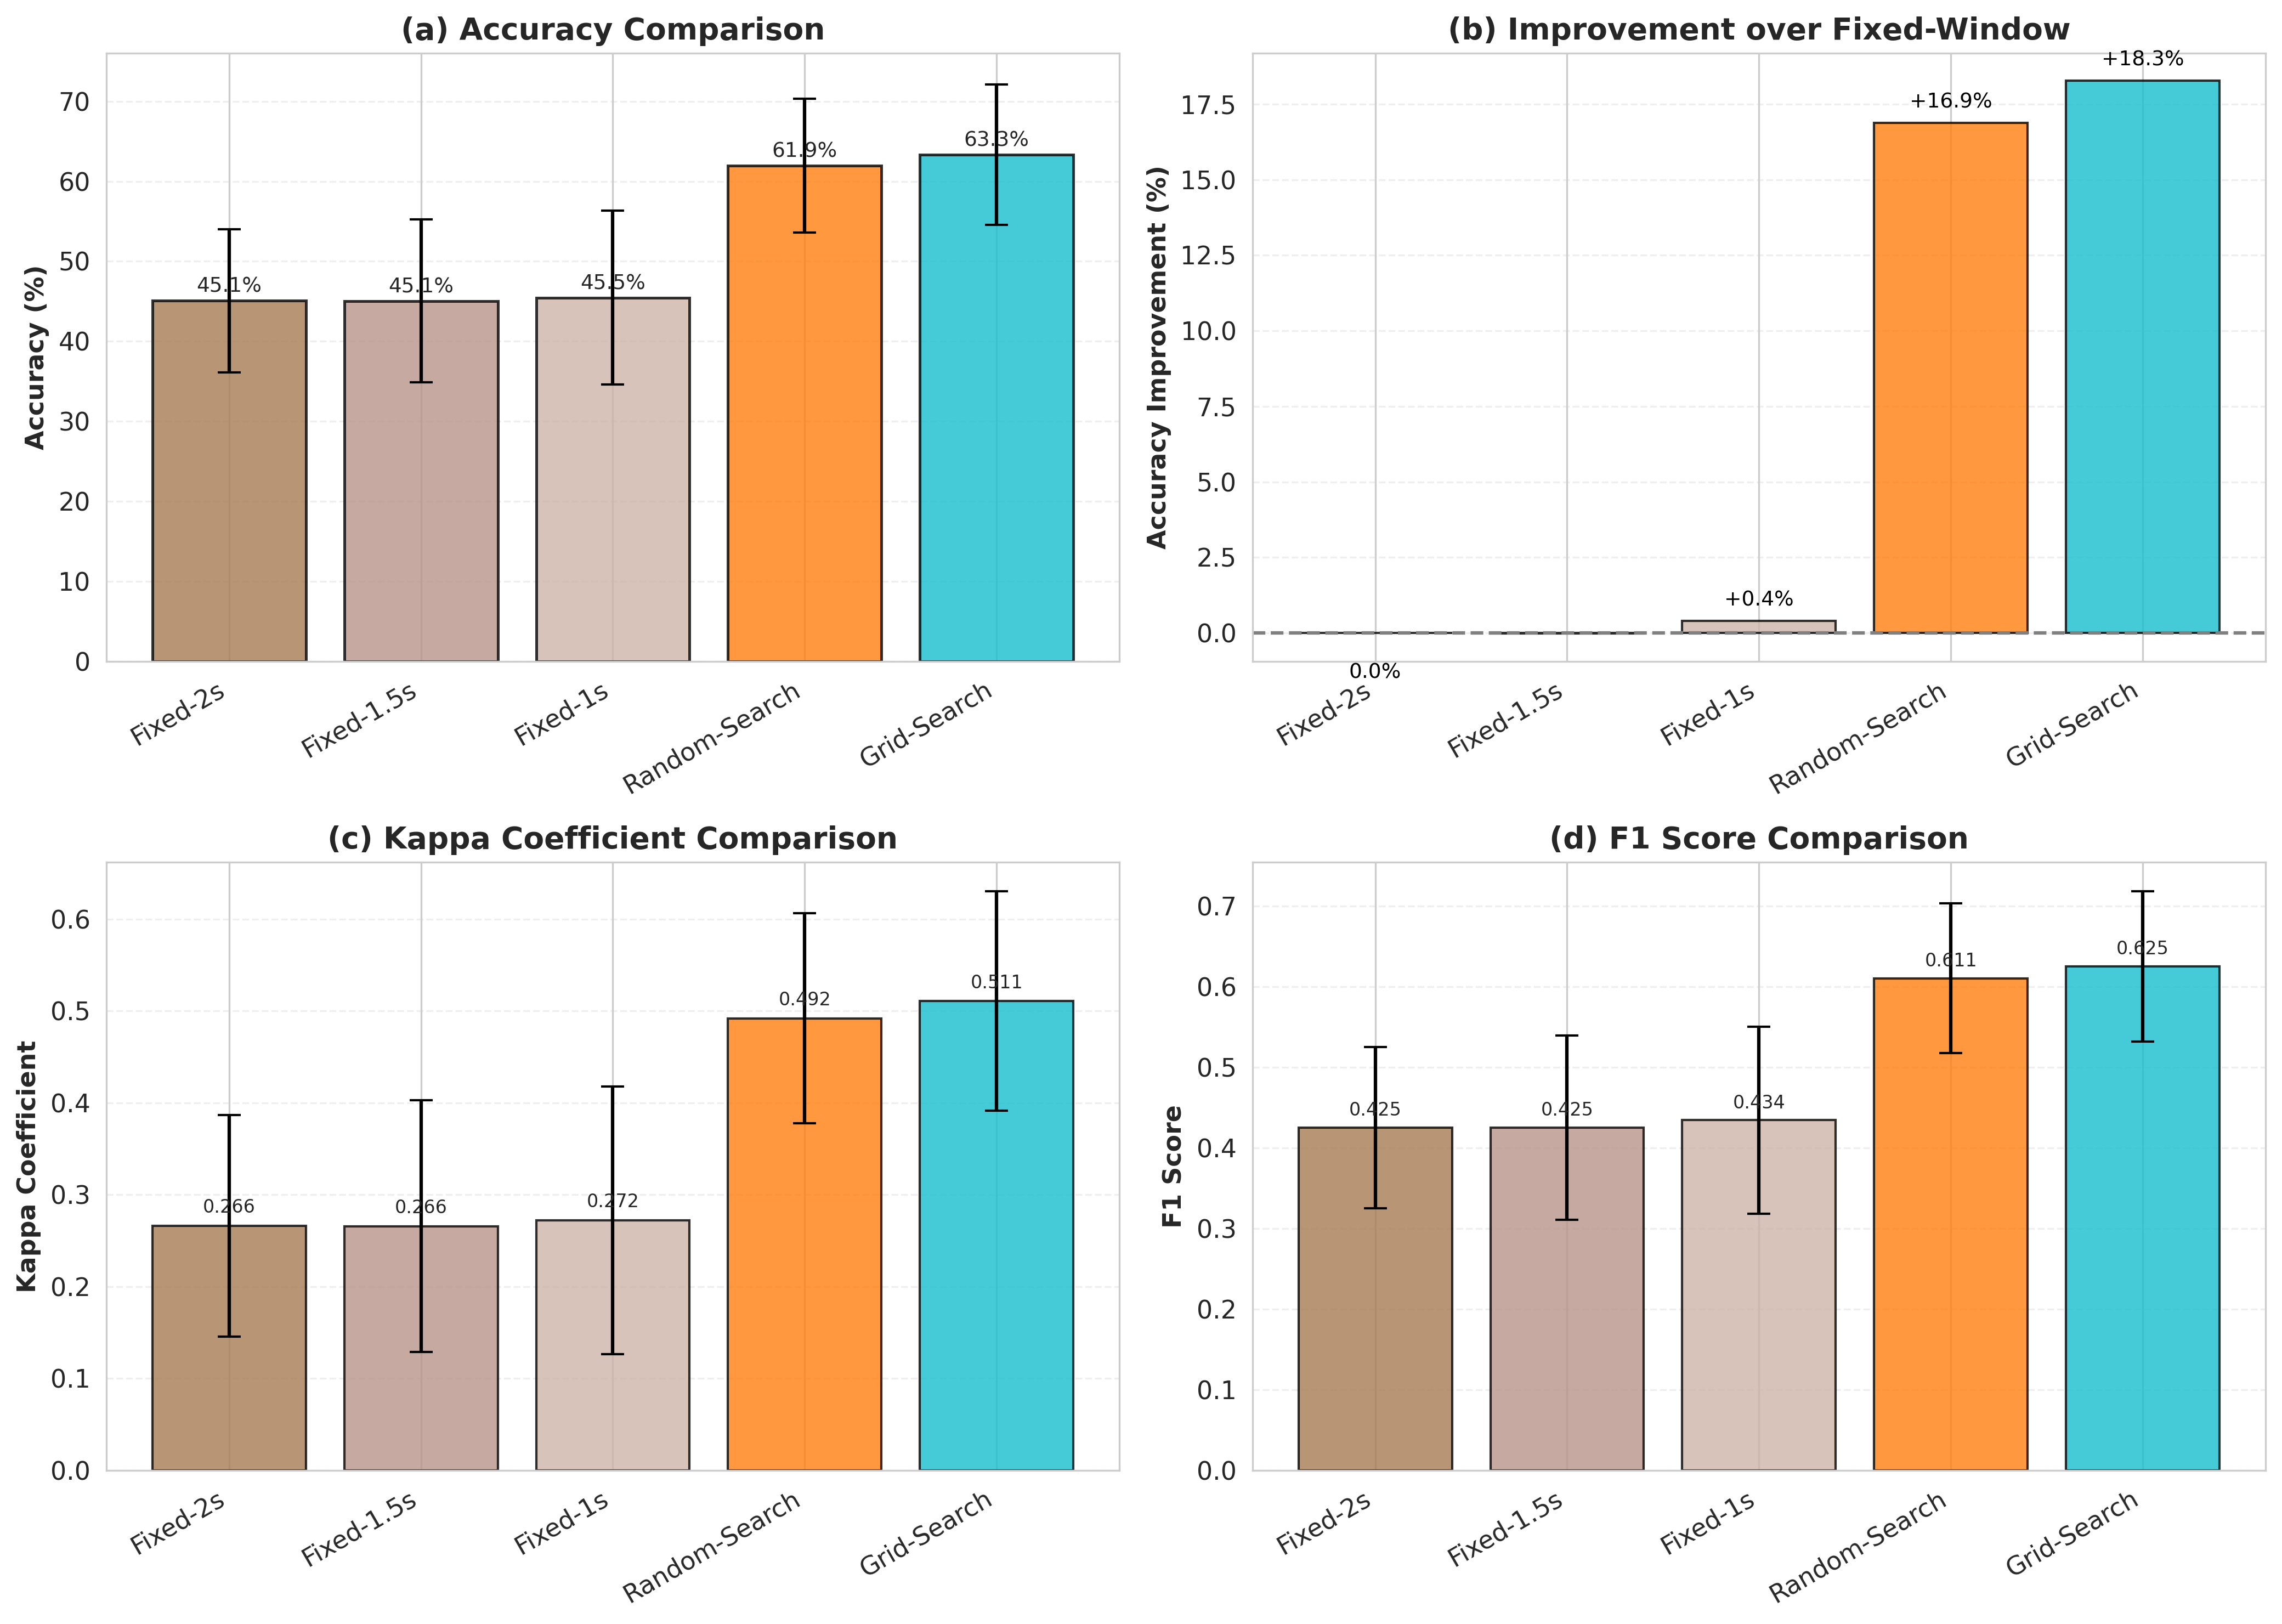
\includegraphics[width=0.85\textwidth]{figures/baseline/01_performance_comparison.png}
    \end{center}
\end{frame}

\begin{frame}{基线方法性能分析}
    \begin{alertblock}{主要发现}
        \footnotesize
        \begin{itemize}
            \item \textbf{准确率}：搜索策略 (61.9\%--63.3\%) 显著优于固定窗口 (约 45\%)
            \item \textbf{提升百分比}：Grid-Search 和 Random-Search 分别实现 +18.3\% 和 +16.9\%
            \item \textbf{Kappa 系数}：搜索策略 (0.49--0.51) 中等一致性，优于固定窗口 (0.27)
            \item \textbf{F1 分数}：搜索策略 (0.61--0.63) 较固定窗口 (0.43) 提升约 44\%
        \end{itemize}
    \end{alertblock}

    \vspace{0.2cm}
    \begin{exampleblock}{结果分析}
        \footnotesize
        搜索优化方法显著优于固定窗口策略。Grid-Search 准确率达 63.35\%，较 Fixed-2s 提升 18.3\%（相对提升 40.6\%）。Kappa 系数从 0.27 提升至 0.51，F1 分数从 0.43 提升至 0.63。这表明\textbf{自适应时间窗口能有效捕捉最优信号片段}，克服固定窗口无法适应 EEG 信号动态变化的局限。
    \end{exampleblock}
\end{frame}

\begin{frame}{基线方法稳定性分析}
    \begin{center}
    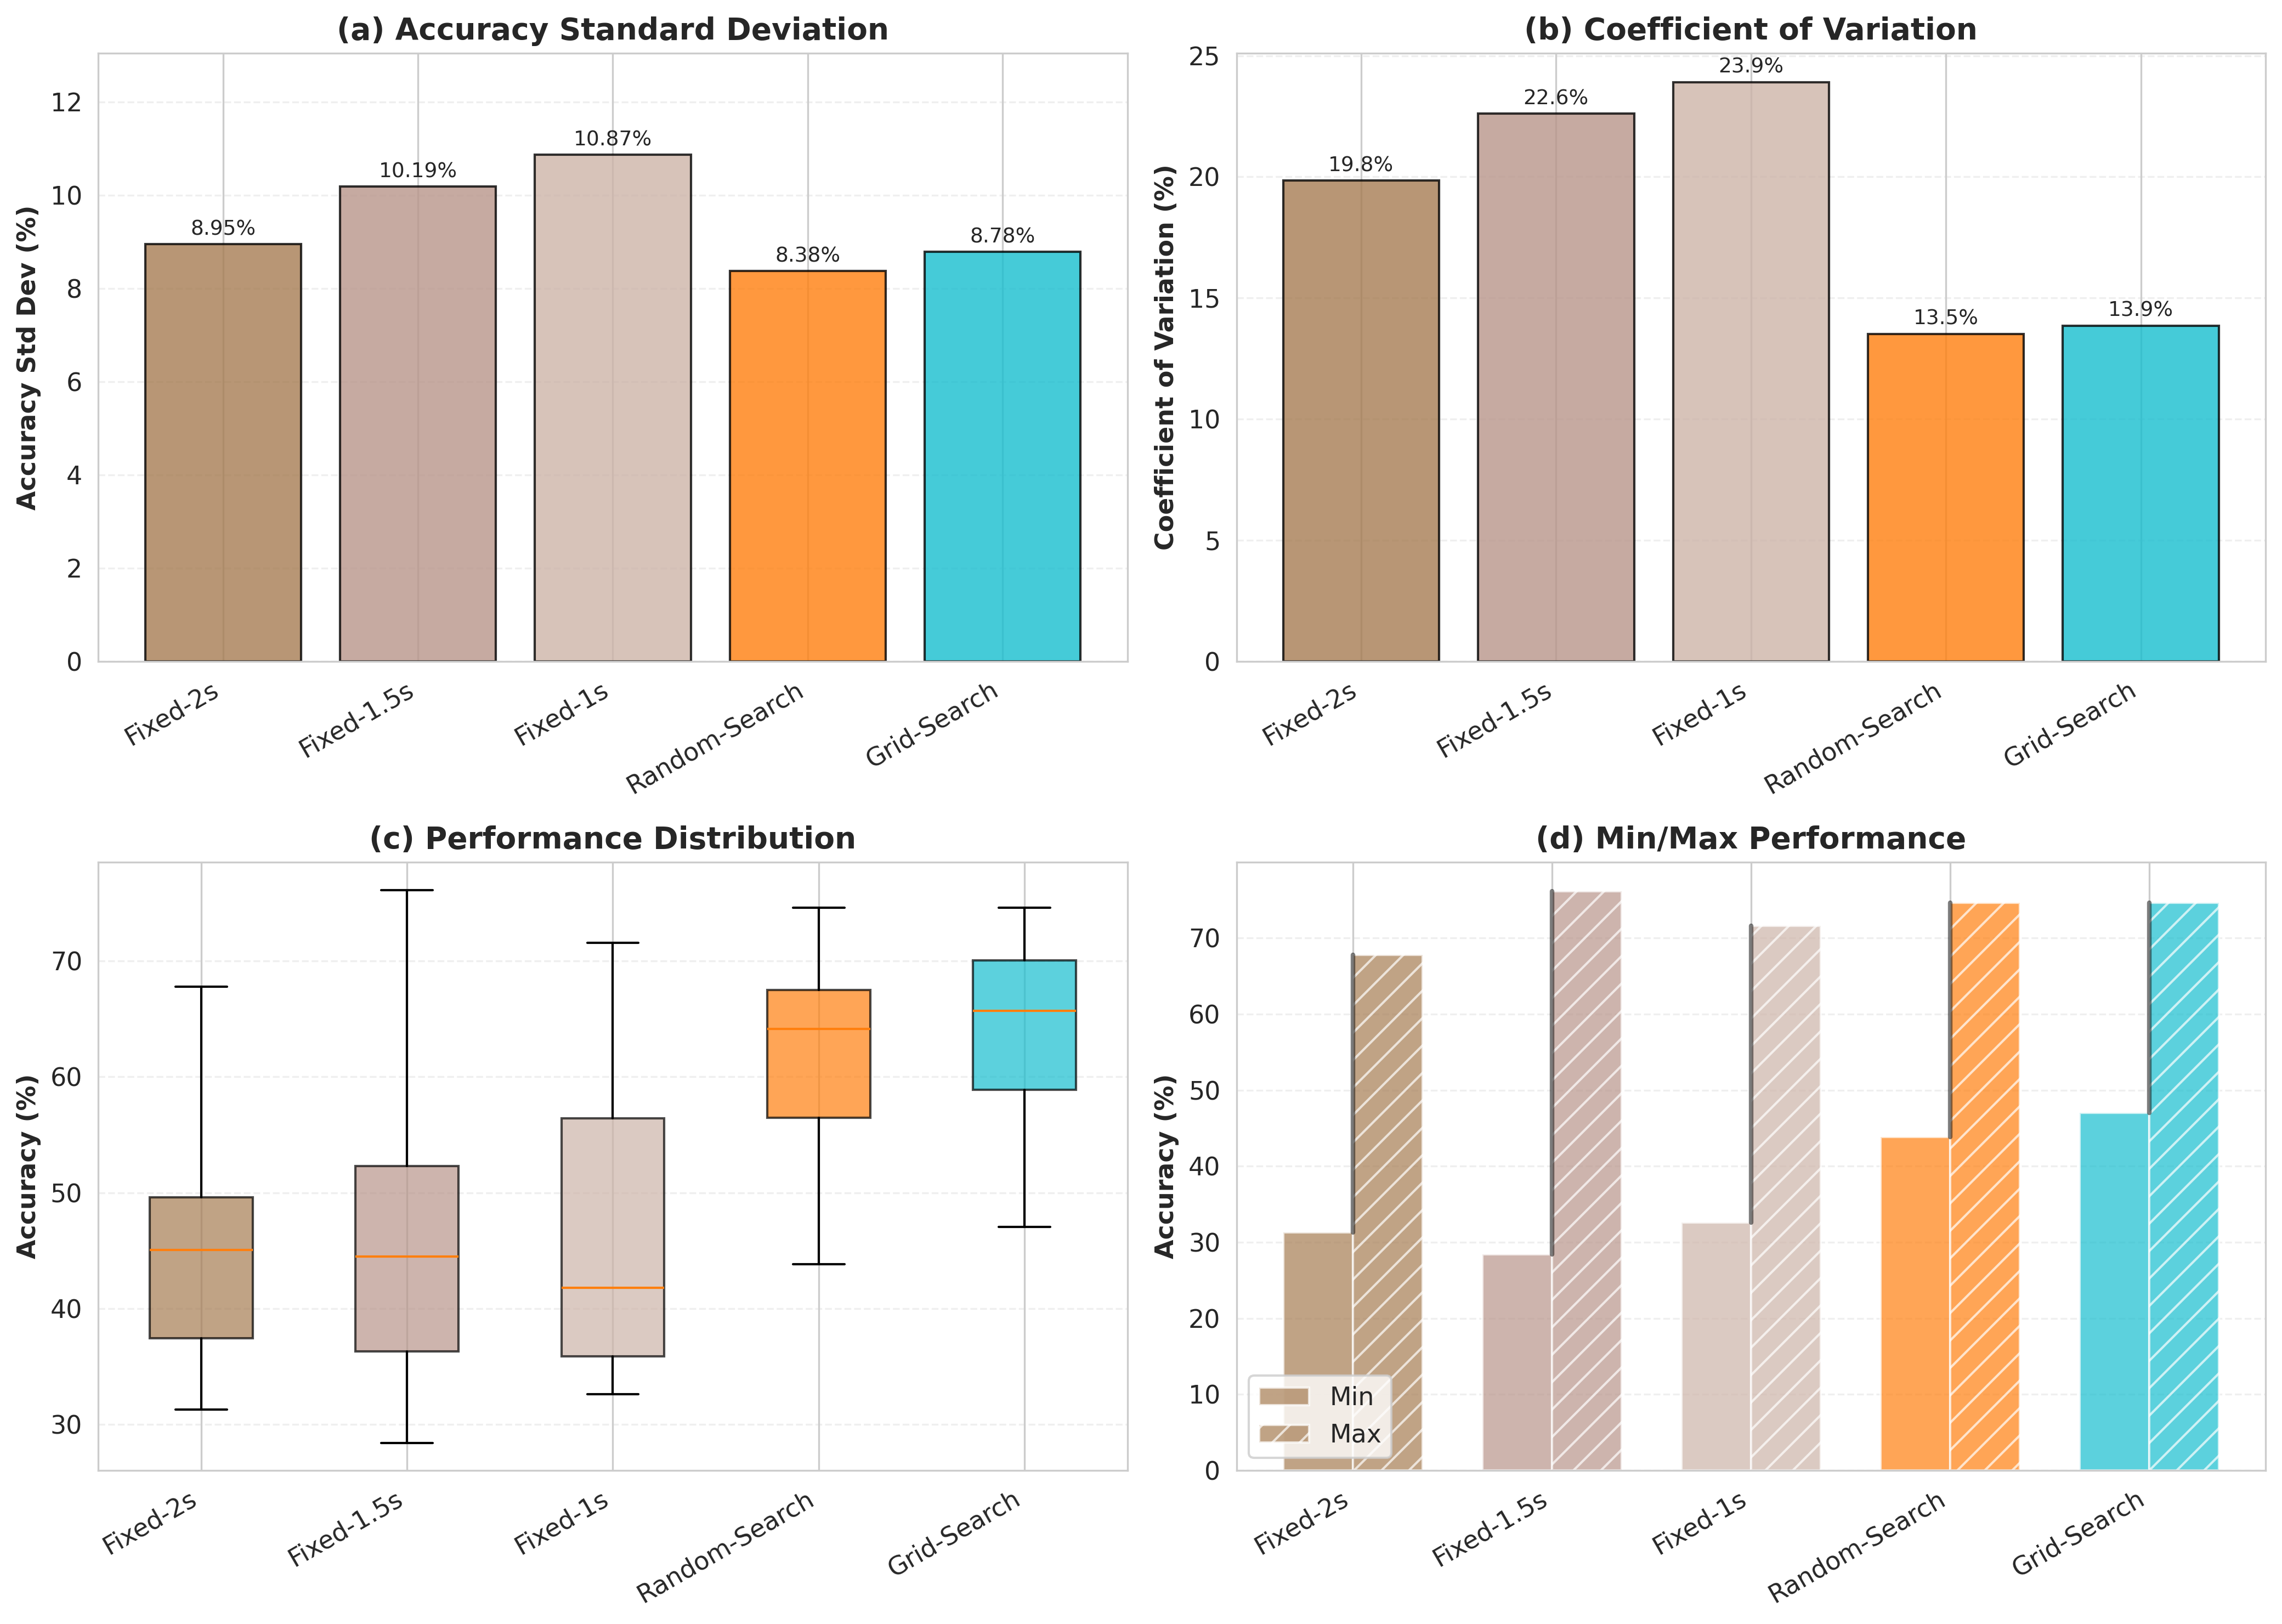
\includegraphics[width=0.85\textwidth]{figures/baseline/01_stability_analysis.png}
    \end{center}
\end{frame}

\begin{frame}{基线方法稳定性分析}
    \begin{exampleblock}{稳定性评估}
        \footnotesize
        \begin{itemize}
            \item \textbf{标准差}：搜索策略显著降低性能波动
            \item \textbf{变异系数}：搜索策略 (13.5\%--13.9\%) vs 固定窗口 (19.8\%--23.9\%)
            \item \textbf{最小准确率}：搜索方法 (约 47\%) 远高于固定窗口 (28\%--33\%)
            \item \textbf{结论}：搜索策略有效提升性能下限保障
        \end{itemize}
    \end{exampleblock}

    \vspace{0.2cm}
    \begin{alertblock}{结果分析}
        \footnotesize
        尽管搜索方法的绝对标准差与 Fixed-2s 相近，但其变异系数显著降低（13.5\%--13.9\% vs 19.8\%--23.9\%）。更重要的是，搜索方法的最小准确率（约 47\%）远高于固定窗口（约 28\%--33\%），\textbf{有效避免了极端差性能的出现}，提高了方法的下限保障。
    \end{alertblock}
\end{frame}

\begin{frame}{各被试准确率分布}
    \begin{center}
    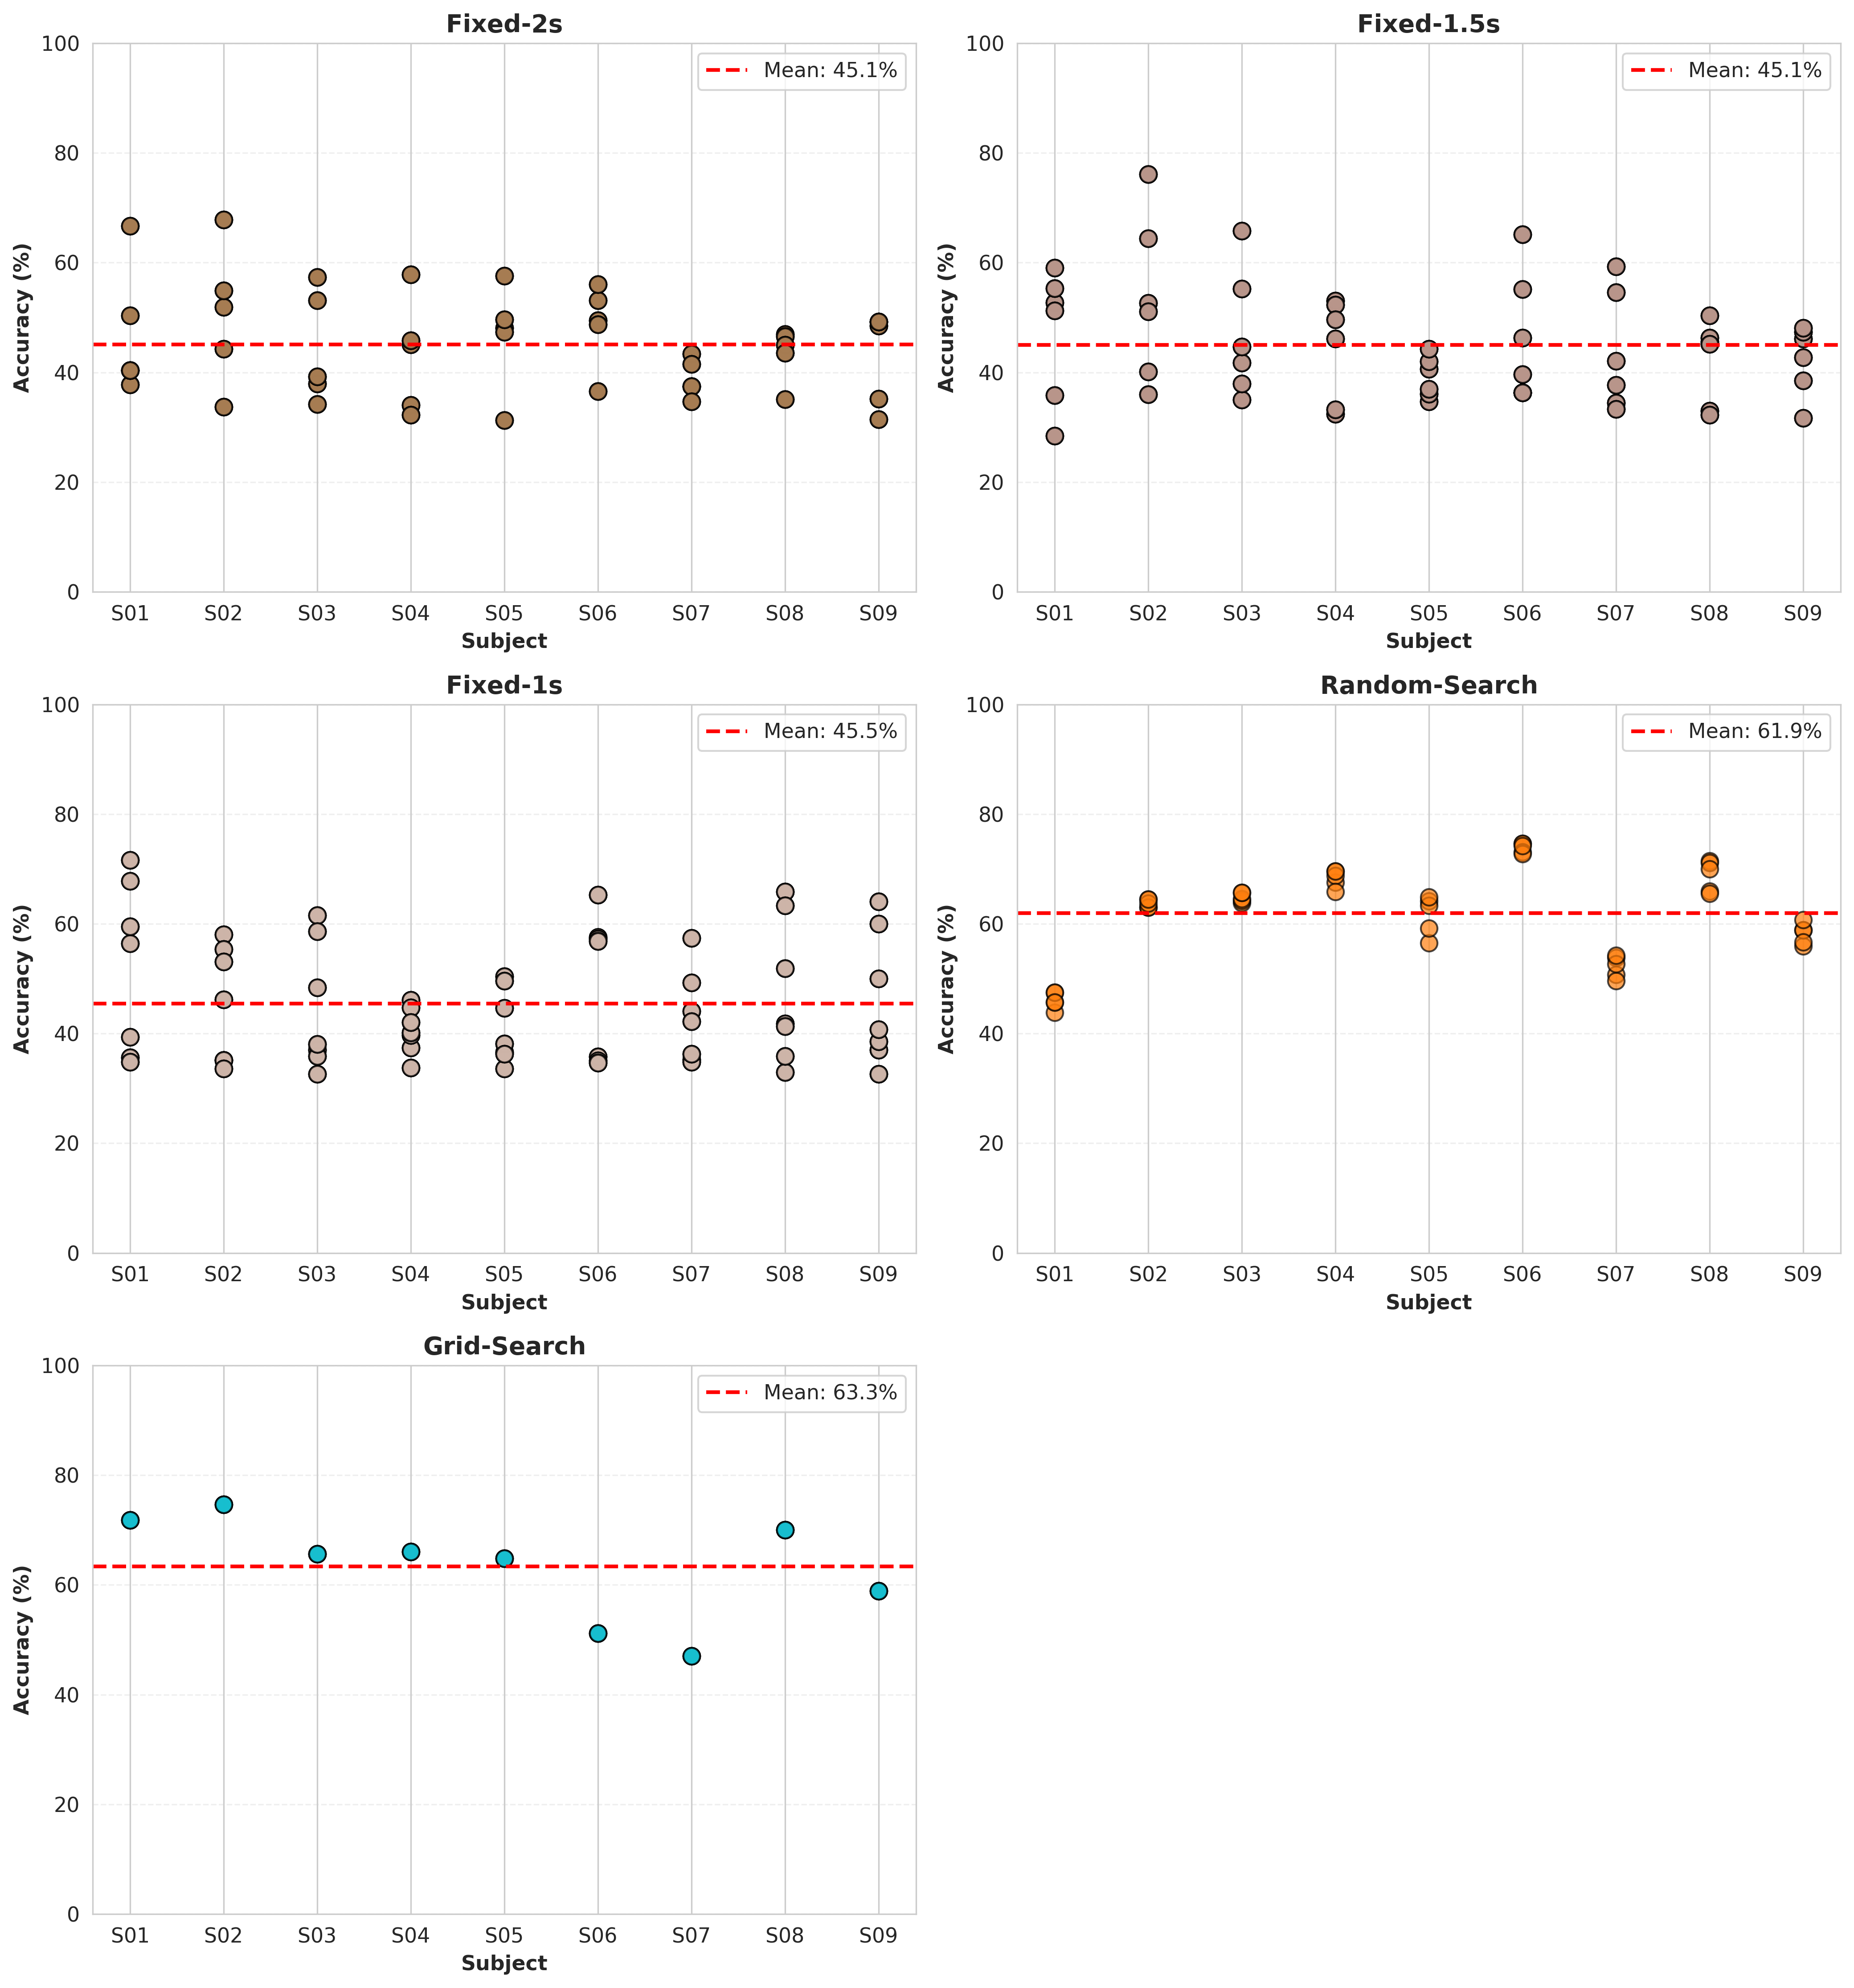
\includegraphics[width=0.6\textwidth]{figures/baseline/01_subject_distribution.png}
    \end{center}
\end{frame}

\begin{frame}{各被试准确率分布分析}
    \begin{alertblock}{个体差异分析}
        \footnotesize
        \begin{itemize}
            \item \textbf{固定窗口}：被试间差异大 (30\%--70\%)，平均停滞在 45\%
            \item \textbf{Random-Search}：同一被试多次运行高度聚集，均值提升至 61.9\%
            \item \textbf{Grid-Search}：最高平均准确率 63.3\%
            \item \textbf{结论}：搜索策略有效缓解个体差异带来的性能波动
        \end{itemize}
    \end{alertblock}

    \vspace{0.2cm}
    \begin{exampleblock}{结果分析}
        \footnotesize
        固定窗口方法在被试间表现出极大波动（30\%--70\%），而 Random-Search 在同一被试的多次运行中高度一致。这验证了\textbf{个体间神经响应模式的异质性}，搜索策略通过为每个样本独立优化窗口，有效适应了这种差异。
    \end{exampleblock}
\end{frame}

\begin{frame}{基线方法详细对比}
    \begin{center}
    \footnotesize
    \renewcommand{\arraystretch}{1.3}
    \begin{tabular}{lccccc}
        \hline
        \textbf{Method} & \textbf{Accuracy (\%)} & \textbf{Kappa} & \textbf{F1} & \textbf{Std Dev (\%)} & \textbf{CV (\%)} \\
        \hline
        Fixed-2s & 45.08 $\pm$ 8.95 & 0.266 & 0.426 & 8.95 & 19.85 \\
        Fixed-1.5s & 45.05 $\pm$ 10.19 & 0.266 & 0.425 & 10.19 & 22.61 \\
        Fixed-1s & 45.47 $\pm$ 10.87 & 0.272 & 0.434 & 10.87 & 23.91 \\
        Random-Search & 61.95 $\pm$ 8.38 & 0.492 & 0.611 & 8.38 & 13.52 \\
        Grid-Search & \textbf{63.35 $\pm$ 8.78} & \textbf{0.511} & \textbf{0.625} & 8.78 & 13.86 \\
        \hline
    \end{tabular}
    \end{center}
\end{frame}

\begin{frame}{基线方法结果分析}
    \begin{alertblock}{结果分析}
        \footnotesize
        \begin{itemize}
            \item Grid-Search 准确率达 63.35\%，较 Fixed-2s 提升 18.3\%
            \item Kappa 系数从 0.27 提升至 0.51，F1 从 0.43 提升至 0.63
            \item 搜索策略变异系数显著降低，有效避免极端差性能
        \end{itemize}
    \end{alertblock}

    \vspace{0.2cm}
    \begin{exampleblock}{搜索策略比较}
        \footnotesize
        Grid-Search 略优于 Random-Search（+1.4\%），但差异微小（< 2.3\%）。考虑到 Random-Search 的计算效率优势，\textbf{在实时 BCI 系统中可能更具实用价值}。三种固定窗口长度性能几乎相同（45.05\%--45.47\%），表明\textbf{简单调整窗口长度无法解决固定窗口的固有局限}，自适应策略是必然选择。
    \end{exampleblock}
\end{frame}

% ============================================================================
% Q-Learning 方法与基线方法对比
% ============================================================================
\subsection{Q-Learning 方法与基线方法对比}

\begin{frame}{Q-Learning 与基线方法性能对比}
    \begin{center}
    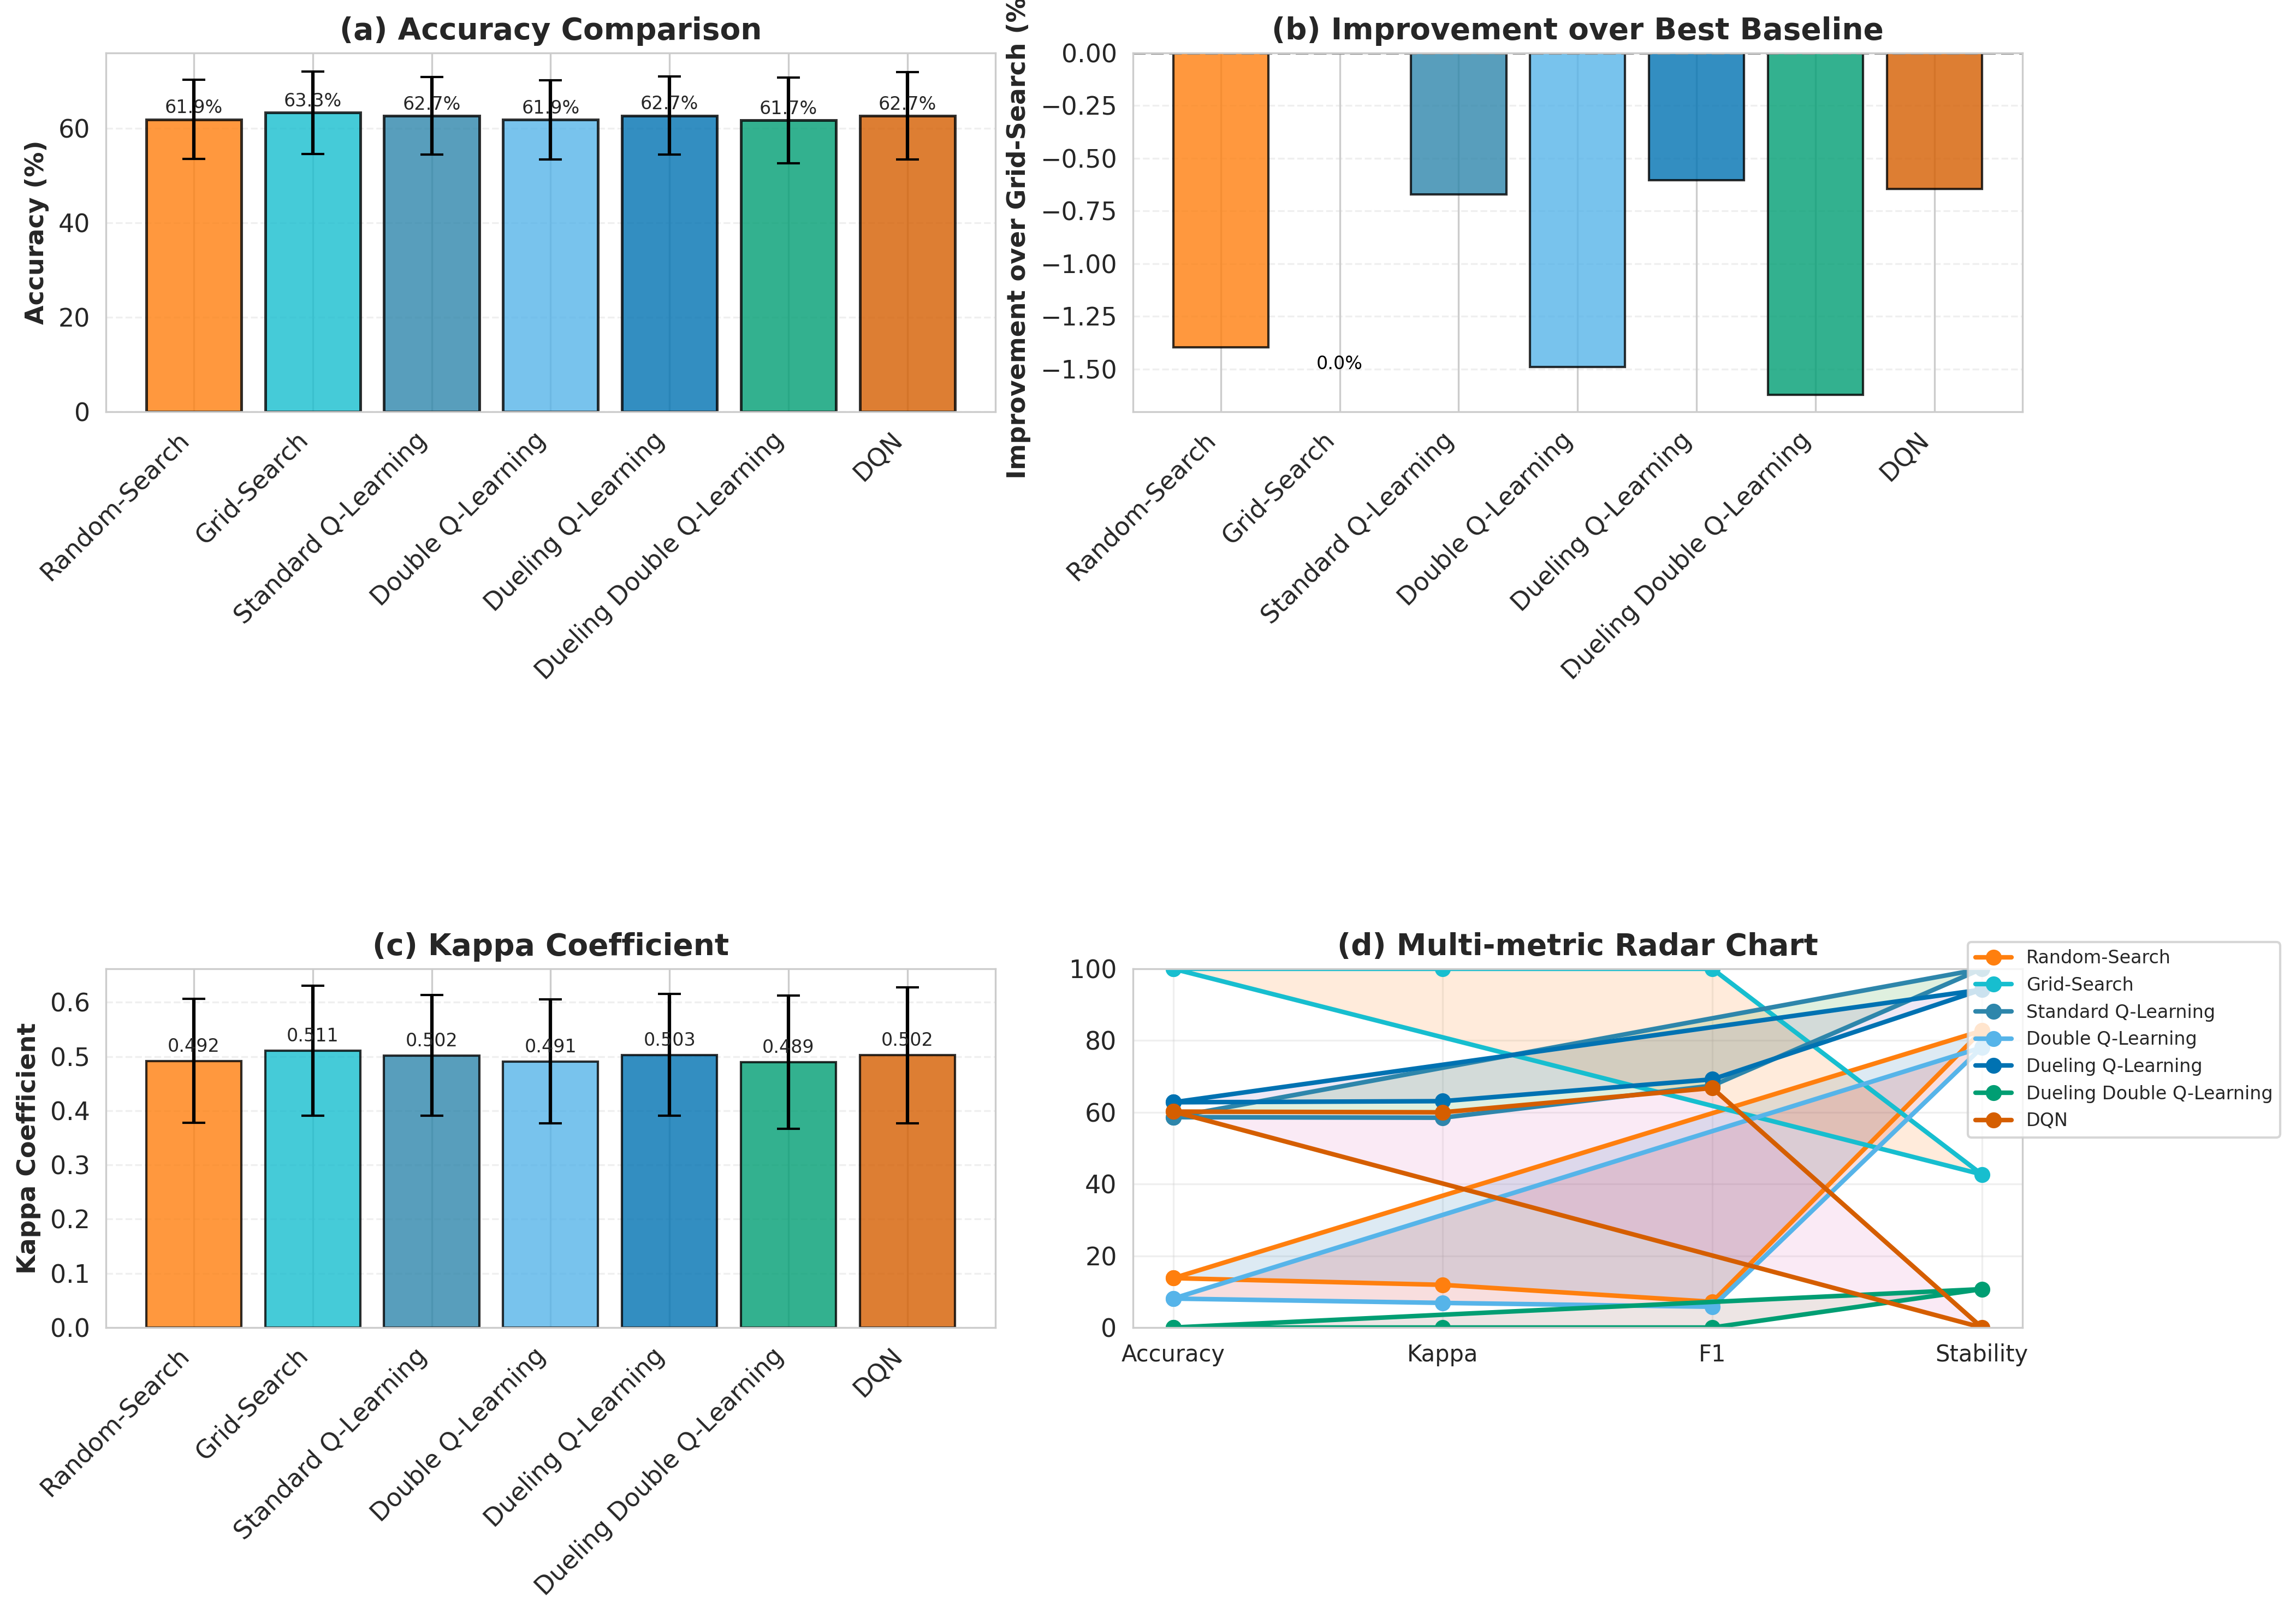
\includegraphics[width=0.85\textwidth]{figures/q_vs_baseline/02_performance_comparison.png}
    \end{center}
\end{frame}

\begin{frame}{Q-Learning 与基线方法性能分析}
    \begin{exampleblock}{性能对比}
        \footnotesize
        \begin{itemize}
            \item \textbf{准确率}：所有方法相近 (61.7\%--63.3\%)，Grid-Search 略居首位
            \item \textbf{相对改进}：强化学习方法略低于 Grid-Search (-0.6\% 至 -1.6\%)
            \item \textbf{Kappa 系数}：各方法集中在 0.49--0.51，一致性水平相当
            \item \textbf{雷达图}：Grid-Search 在准确率和 F1 最优，强化学习在稳定性略有优势
        \end{itemize}
    \end{exampleblock}

    \vspace{0.2cm}
    \begin{alertblock}{结果分析}
        \footnotesize
        Grid-Search 以 63.3\% 的准确率位居首位，所有强化学习方法的性能均略低于 Grid-Search（-0.6\% 至 -1.6\%），Random-Search 差距为 -1.4\%。各方法 Kappa 系数集中在 0.49--0.51 之间，分类一致性水平相当。实验结果表明，强化学习方法能够以较低的计算成本达到与网格搜索相近的性能水平，为实时自适应时间窗口选择提供了可行方案。
    \end{alertblock}
\end{frame}

\begin{frame}{统计显著性分析}
    \begin{center}
    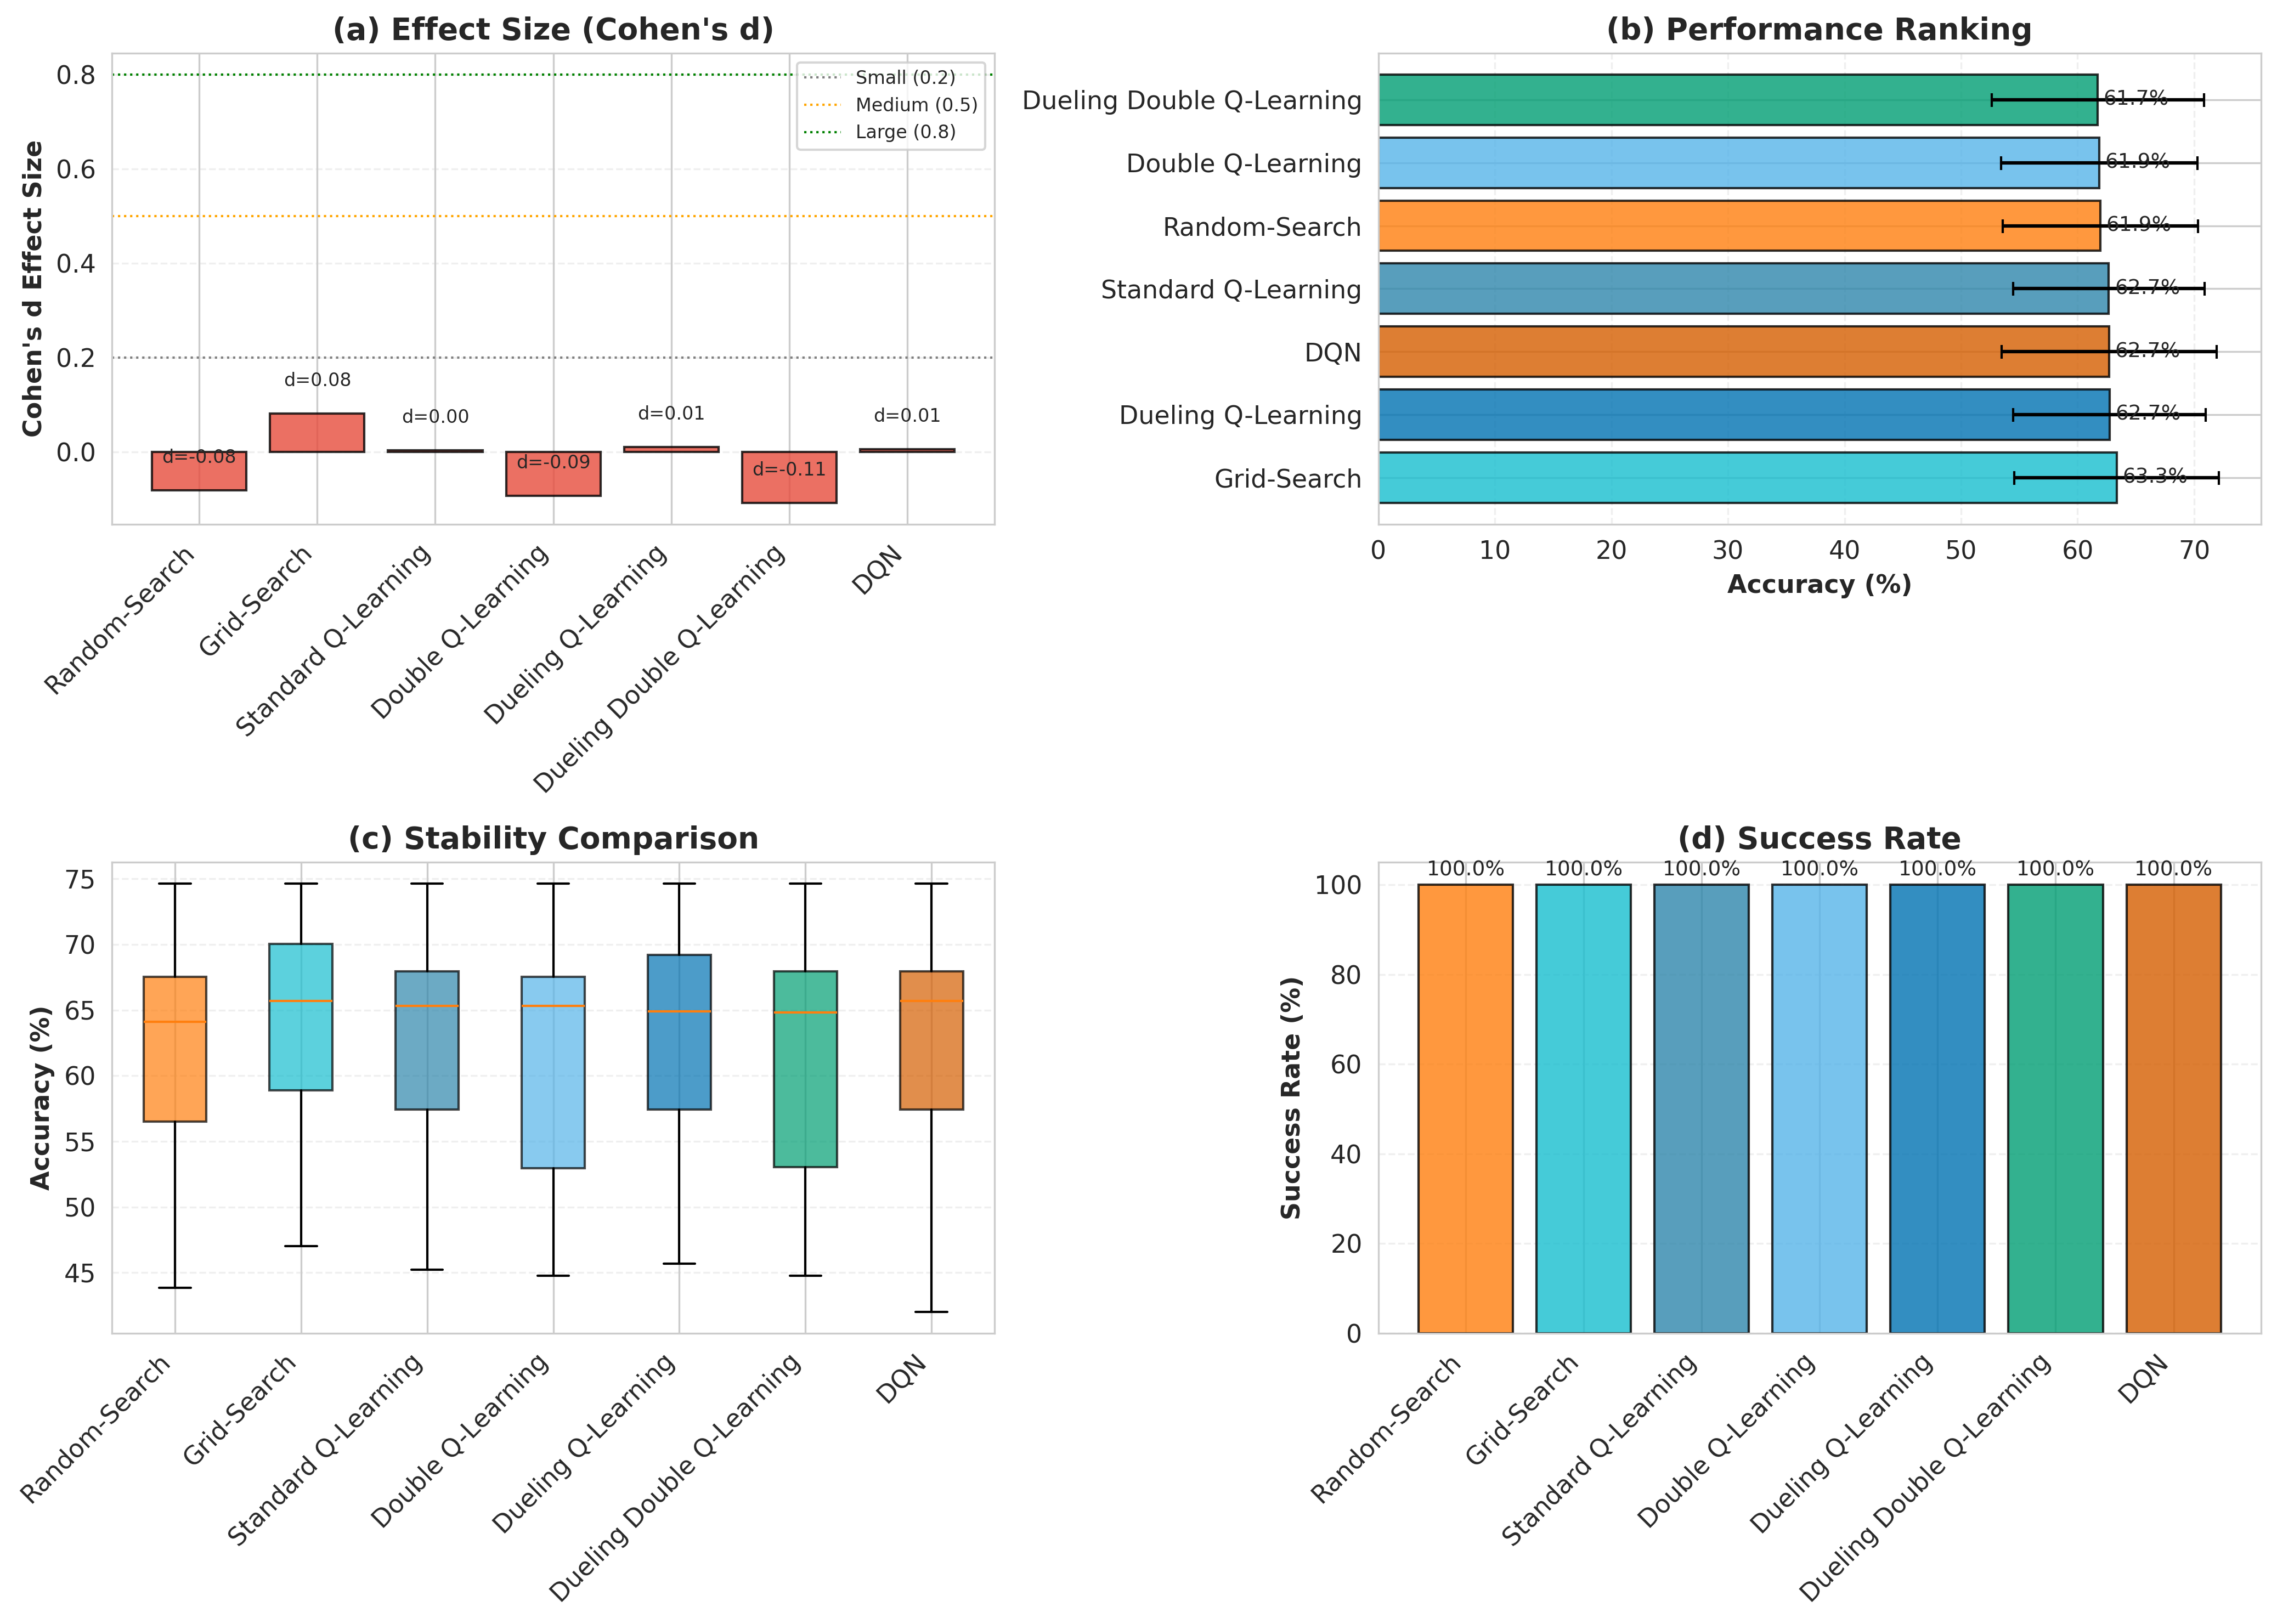
\includegraphics[width=0.85\textwidth]{figures/q_vs_baseline/02_statistical_analysis.png}
    \end{center}
\end{frame}

\begin{frame}{统计显著性分析}
    \begin{alertblock}{统计评估}
        \footnotesize
        \begin{itemize}
            \item \textbf{效应量}：所有方法效应量远小于小效应阈值 ($|d| < 0.2$)
            \item \textbf{性能排名}：Grid-Search (63.3\%) 第一，Q-Learning 变体 (62.7\%) 并列第二
            \item \textbf{稳定性}：各方法准确率分布范围相近 (45\%--75\%)
            \item \textbf{成功率}：所有方法均达 100\% 成功率
        \end{itemize}
    \end{alertblock}

    \vspace{0.2cm}
    \begin{exampleblock}{结果分析}
        \footnotesize
        所有 Q-Learning 方法与 Grid-Search 的 Cohen's d 值均远小于小效应阈值（$|d| < 0.2$），其中 Dueling Double Q-Learning 的效应量最大（$d=-0.11$）。这表明\textbf{尽管 Grid-Search 在数值上略优，但差异在统计学上不显著}，Q-Learning 方法可视为与 Grid-Search 性能等效。
    \end{exampleblock}
\end{frame}

\begin{frame}{时间窗选择模式分析}
    \begin{center}
    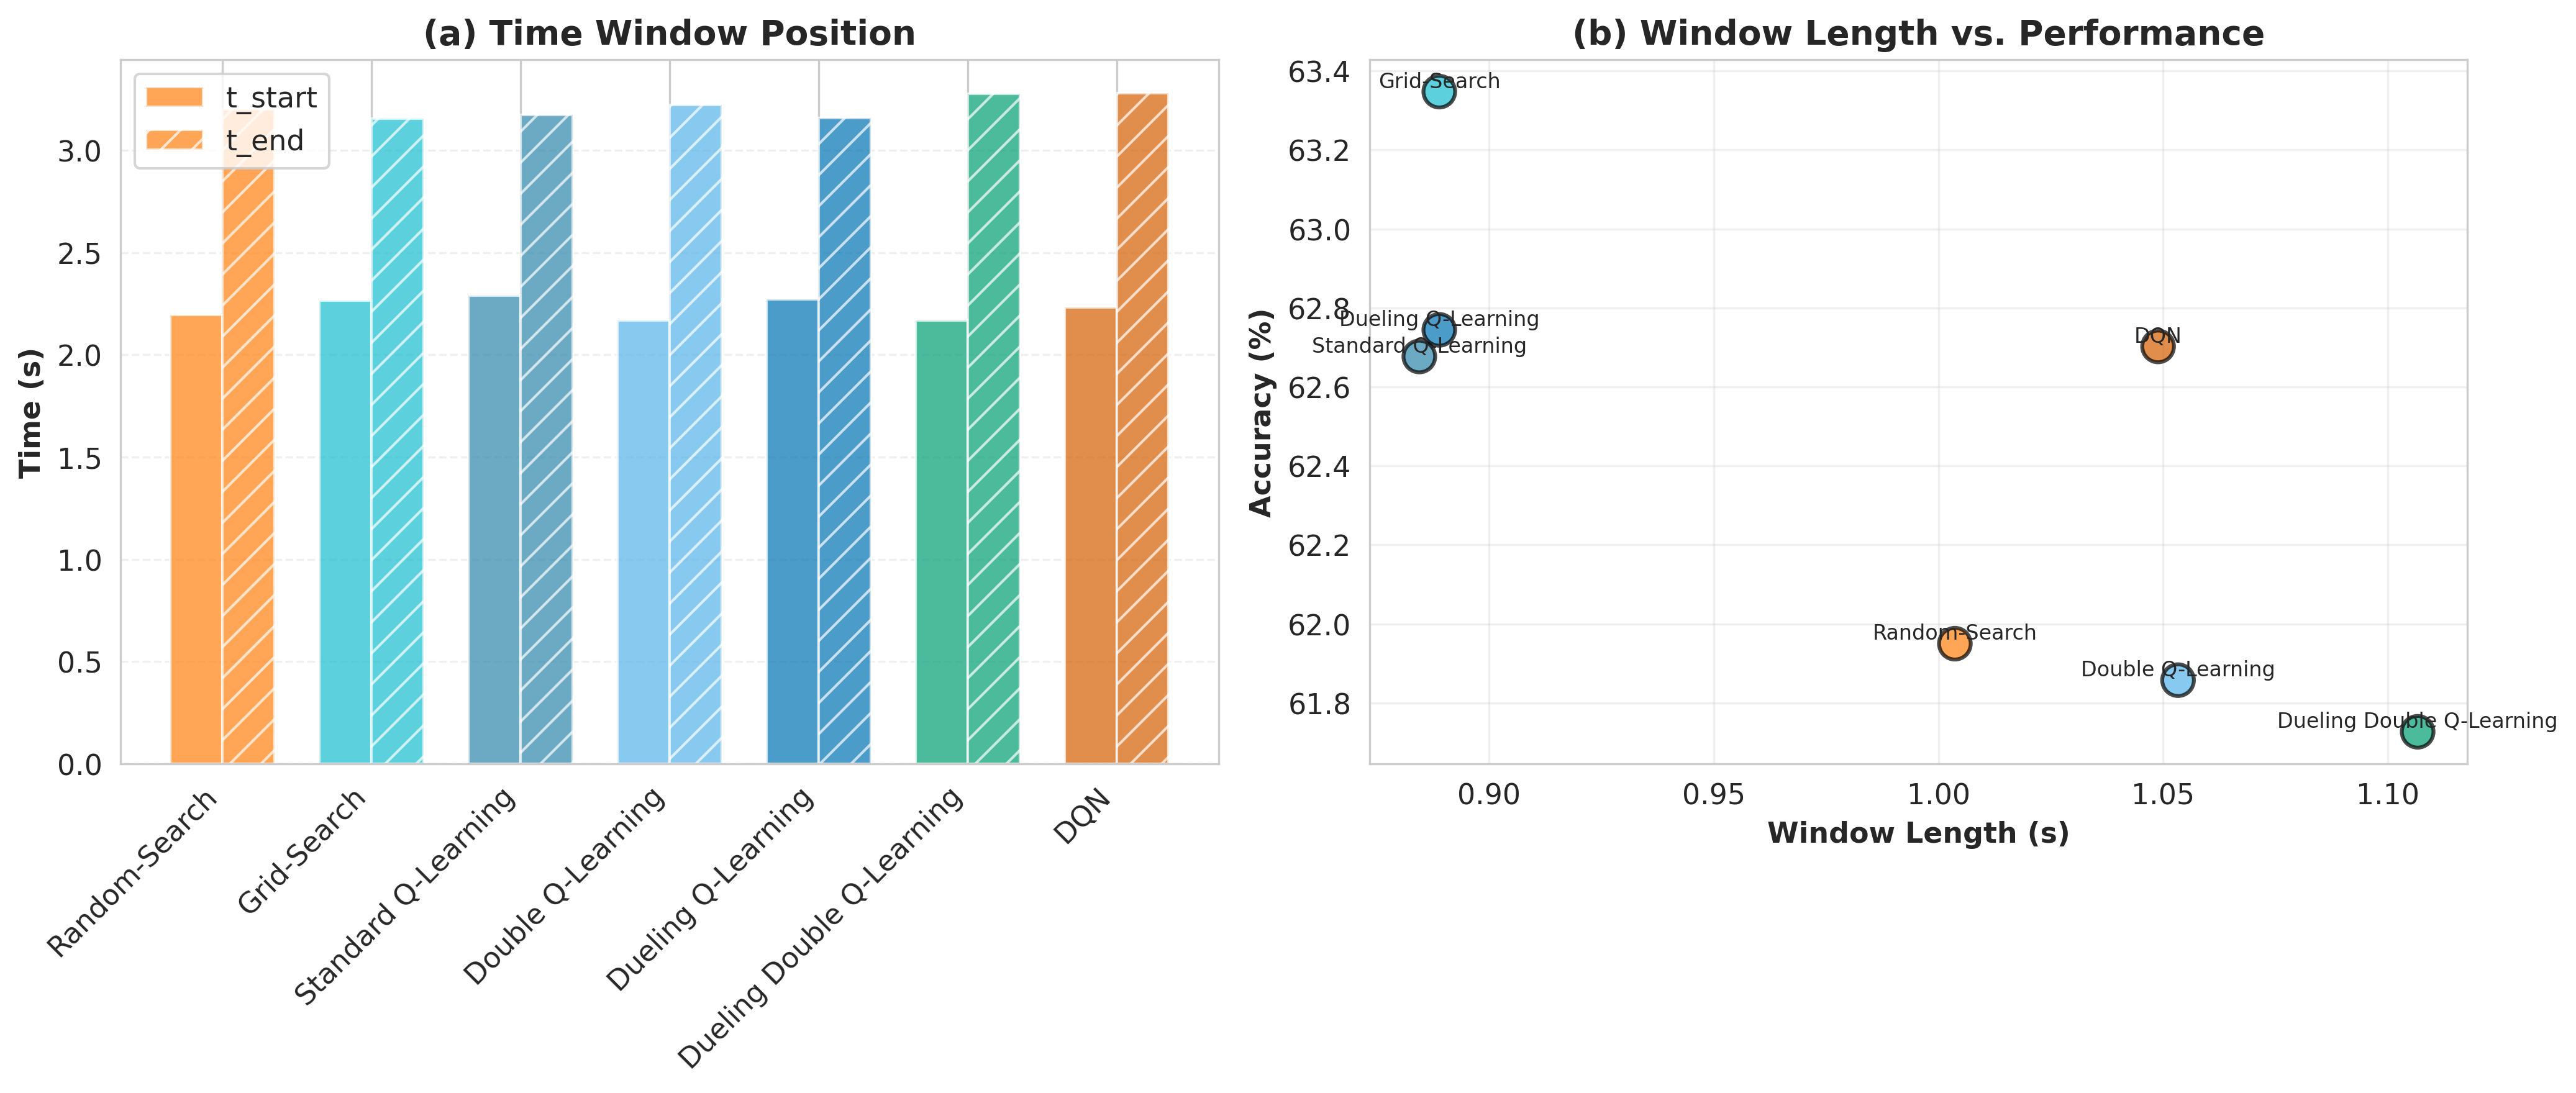
\includegraphics[width=0.85\textwidth]{figures/q_vs_baseline/02_window_performance.png}
    \end{center}
\end{frame}

\begin{frame}{时间窗选择模式分析}
    \begin{exampleblock}{时间窗分析}
        \footnotesize
        \begin{itemize}
            \item \textbf{位置分布}：所有方法倾向选择试验后期 ($t_{start} \approx 2.2$s, $t_{end} \approx 3.3$s)
            \item \textbf{关键发现}：运动想象关键神经特征主要分布在 trials 后半段
            \item \textbf{窗口长度与性能}：显著负相关，较短窗口 (约 0.9s) 准确率更高
            \item \textbf{结论}：精简时间窗口有助于减少噪声干扰并提升分类性能
        \end{itemize}
    \end{exampleblock}

    \vspace{0.2cm}
    \begin{alertblock}{结果分析}
        \footnotesize
        所有方法均倾向于选择试验后期的时间片段（$t_{start} \approx 2.2$s，$t_{end} \approx 3.3$s），验证了运动想象关键特征分布在 trials 后半段的假设。此外，窗口长度与性能呈负相关趋势，较短窗口（约 0.9s）比较长窗口（>1.0s）准确率更高，表明\textbf{精简窗口有助于减少噪声干扰}。Q-Learning 代理在训练过程中逐渐收敛至这一最优窗口范围，体现了其学习能力。
    \end{alertblock}
\end{frame}

\begin{frame}{Q-Learning 方法详细对比}
    \begin{center}
    \footnotesize
    \renewcommand{\arraystretch}{1.3}
    \begin{tabular}{lcccc}
        \hline
        \textbf{Method} & \textbf{Accuracy (\%)} & \textbf{Kappa} & \textbf{F1} & \textbf{Std Dev (\%)} \\
        \hline
        Random-Search & 61.95 $\pm$ 8.38 & 0.492 & 0.611 & 8.38 \\
        Grid-Search & \textbf{63.35 $\pm$ 8.78} & \textbf{0.511} & \textbf{0.625} & 8.78 \\
        Standard Q-Learning & 62.68 $\pm$ 8.20 & 0.502 & 0.620 & \textbf{8.20} \\
        Double Q-Learning & 61.86 $\pm$ 8.42 & 0.491 & 0.610 & 8.42 \\
        Dueling Q-Learning & 62.74 $\pm$ 8.26 & 0.503 & 0.620 & 8.26 \\
        Dueling Double Q-Learning & 61.73 $\pm$ 9.11 & 0.489 & 0.609 & 9.11 \\
        DQN & 62.70 $\pm$ 9.21 & 0.502 & 0.620 & 9.21 \\
        \hline
    \end{tabular}
    \end{center}
\end{frame}

\begin{frame}{Q-Learning 方法结果分析}
    \begin{alertblock}{结果分析}
        \footnotesize
        \begin{itemize}
            \item Standard Q-Learning 和 Dueling Q-Learning 表现最佳 (62.7\%)
            \item 与 Grid-Search 差距仅 0.6\%--1.6\%，统计上不显著
            \item Standard Q-Learning 稳定性最优 (Std Dev = 8.20\%)
        \end{itemize}
    \end{alertblock}

    \vspace{0.2cm}
    \begin{exampleblock}{稳定性与计算效率}
        \footnotesize
        从标准差来看，Standard Q-Learning（8.20\%）和 Dueling Q-Learning（8.26\%）的稳定性略优于 Grid-Search（8.78\%）和 Random-Search（8.38\%）。更重要的是，Q-Learning 方法在推理阶段仅需单次前向传播即可确定时间窗口，而 Grid-Search 需要遍历所有候选窗口组合。考虑到两者性能差异不显著（$< 1.6\%$），\textbf{Q-Learning 方法在实时 BCI 系统中具有明显的计算效率优势}。
    \end{exampleblock}
\end{frame}

% ============================================================================
% 表格型 Q-Learning 与 DQN 对比
% ============================================================================
\subsection{表格型 Q-Learning 与 DQN 对比}

\begin{frame}{Q-Learning 变体性能对比}
    \begin{center}
    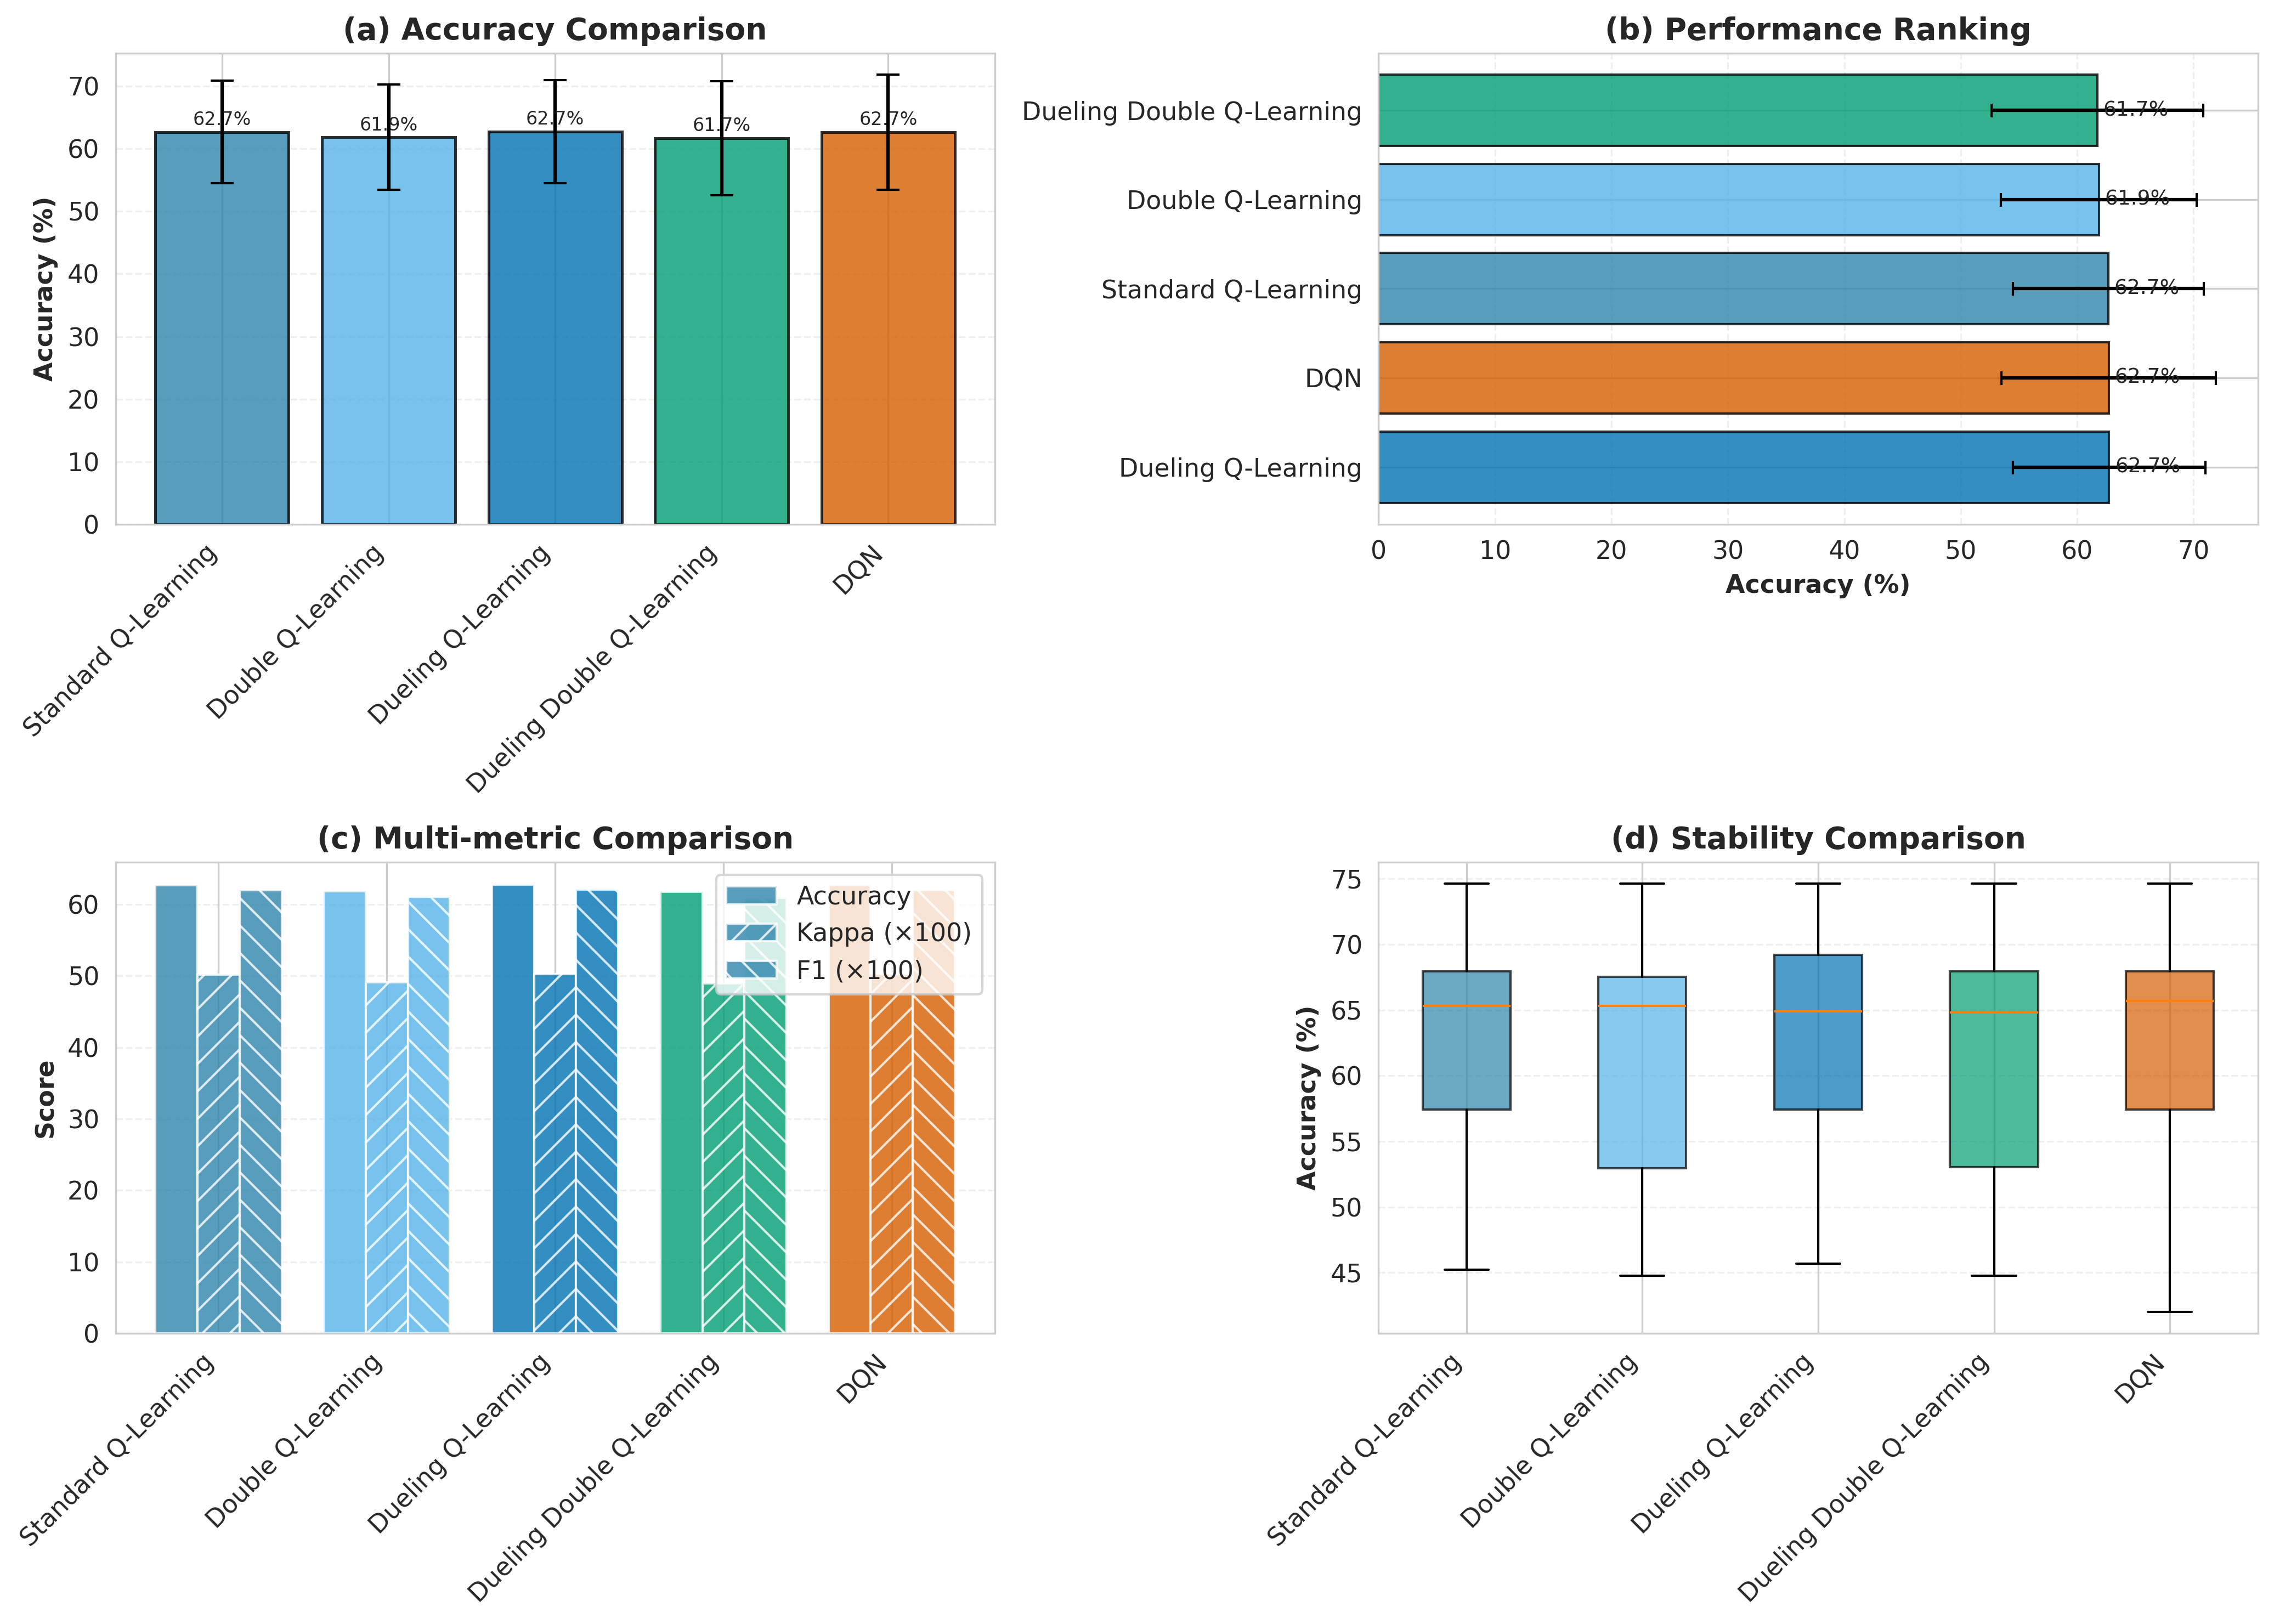
\includegraphics[width=0.85\textwidth]{figures/q_internal/03_performance_comparison.png}
    \end{center}
\end{frame}

\begin{frame}{Q-Learning 变体性能分析}
    \begin{exampleblock}{变体对比}
        \footnotesize
        \begin{itemize}
            \item \textbf{准确率}：各变体高度接近 (61.7\%--62.7\%)
            \item \textbf{最佳性能}：Standard Q-Learning、Dueling Q-Learning 和 DQN 并列 (62.7\%)
            \item \textbf{多指标}：所有变体在准确率、Kappa、F1 上表现一致
            \item \textbf{结论}：Standard Q-Learning 已足以捕捉策略，复杂变体未带来显著增益
        \end{itemize}
    \end{exampleblock}

    \vspace{0.2cm}
    \begin{alertblock}{结果分析}
        \footnotesize
        各变体性能高度接近（61.7\%--62.7\%），Standard Q-Learning、Dueling Q-Learning 和 DQN 并列最佳（62.7\%）。性能排名进一步确认了 Standard Q-Learning 等三种方法的领先地位，Dueling Double Q-Learning 略低（61.7\%）。多指标综合对比显示，所有变体在各项指标上表现一致，未见特定变体在某项指标上有显著优势。结果表明，在本任务中，\textbf{Standard Q-Learning 已足以捕捉时间窗口选择的策略，复杂的变体改进并未带来显著的性能增益}。
    \end{alertblock}
\end{frame}

\begin{frame}{Table Q-Learning 与 DQN 深度对比}
    \begin{center}
    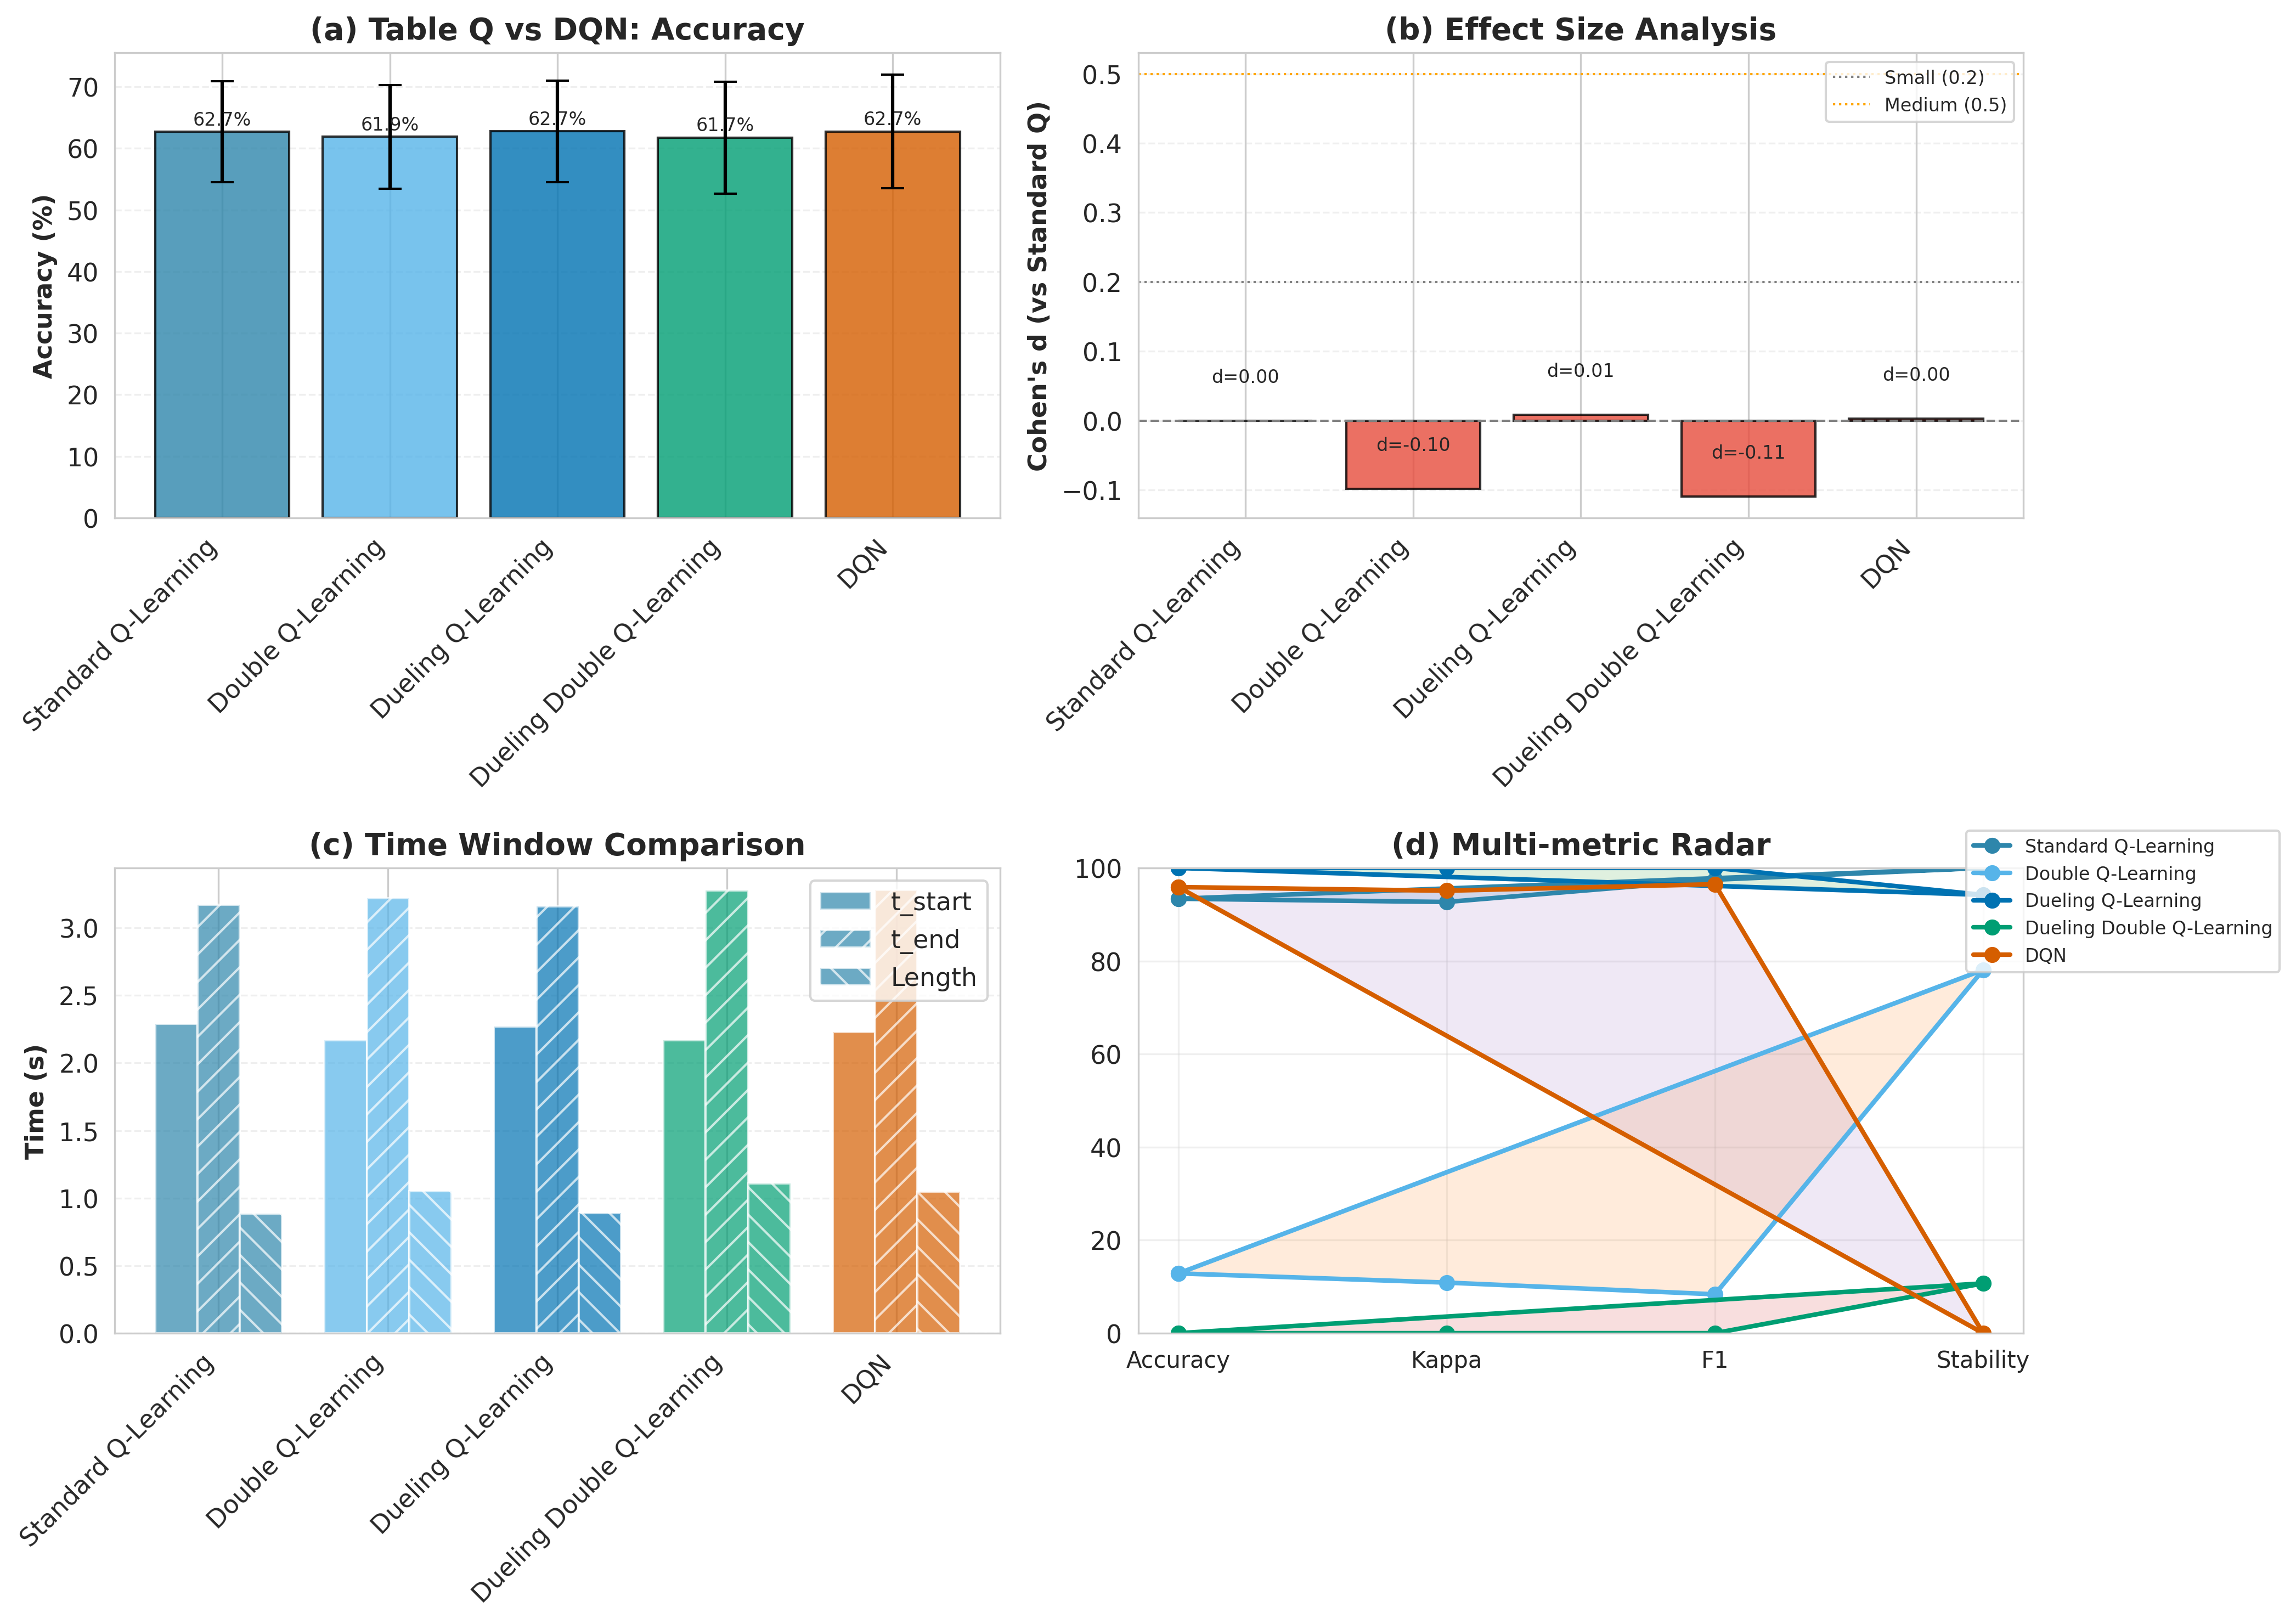
\includegraphics[width=0.85\textwidth]{figures/q_internal/03_table_q_vs_dqn.png}
    \end{center}
\end{frame}

\begin{frame}{Table Q-Learning 与 DQN 深度对比分析}
    \begin{alertblock}{深度对比}
        \footnotesize
        \begin{itemize}
            \item \textbf{准确率}：所有方法高度接近 (61.7\%--62.7\%)
            \item \textbf{效应量}：所有 $|d| < 0.2$，Standard Q 与 DQN 几乎无差异 ($d=0.00$)
            \item \textbf{时间窗}：DQN 选较短窗口 (约 1.0s)，Table Q 分布在 0.9s--1.1s
            \item \textbf{结论}：简单 Table Q-Learning 与复杂 DQN 性能相当
        \end{itemize}
    \end{alertblock}

    \vspace{0.2cm}
    \begin{exampleblock}{结果分析}
        \footnotesize
        所有方法性能高度接近（61.7\%--62.7\%），Standard Q-Learning、Dueling Q-Learning 和 DQN 均达到 62.7\% 的最高准确率。效应量分析显示，所有方法的效应量均远低于小效应阈值（$|d| < 0.2$），其中 Double Q-Learning ($d=-0.10$) 和 Dueling Double Q-Learning ($d=-0.11$) 显示出微小的负效应。结果表明，\textbf{在本任务中，简单的 Table Q-Learning 与复杂的 DQN 性能相当}，说明状态空间离散化策略已足够有效。
    \end{exampleblock}
\end{frame}

\begin{frame}{训练收敛特性分析}
    \begin{center}
    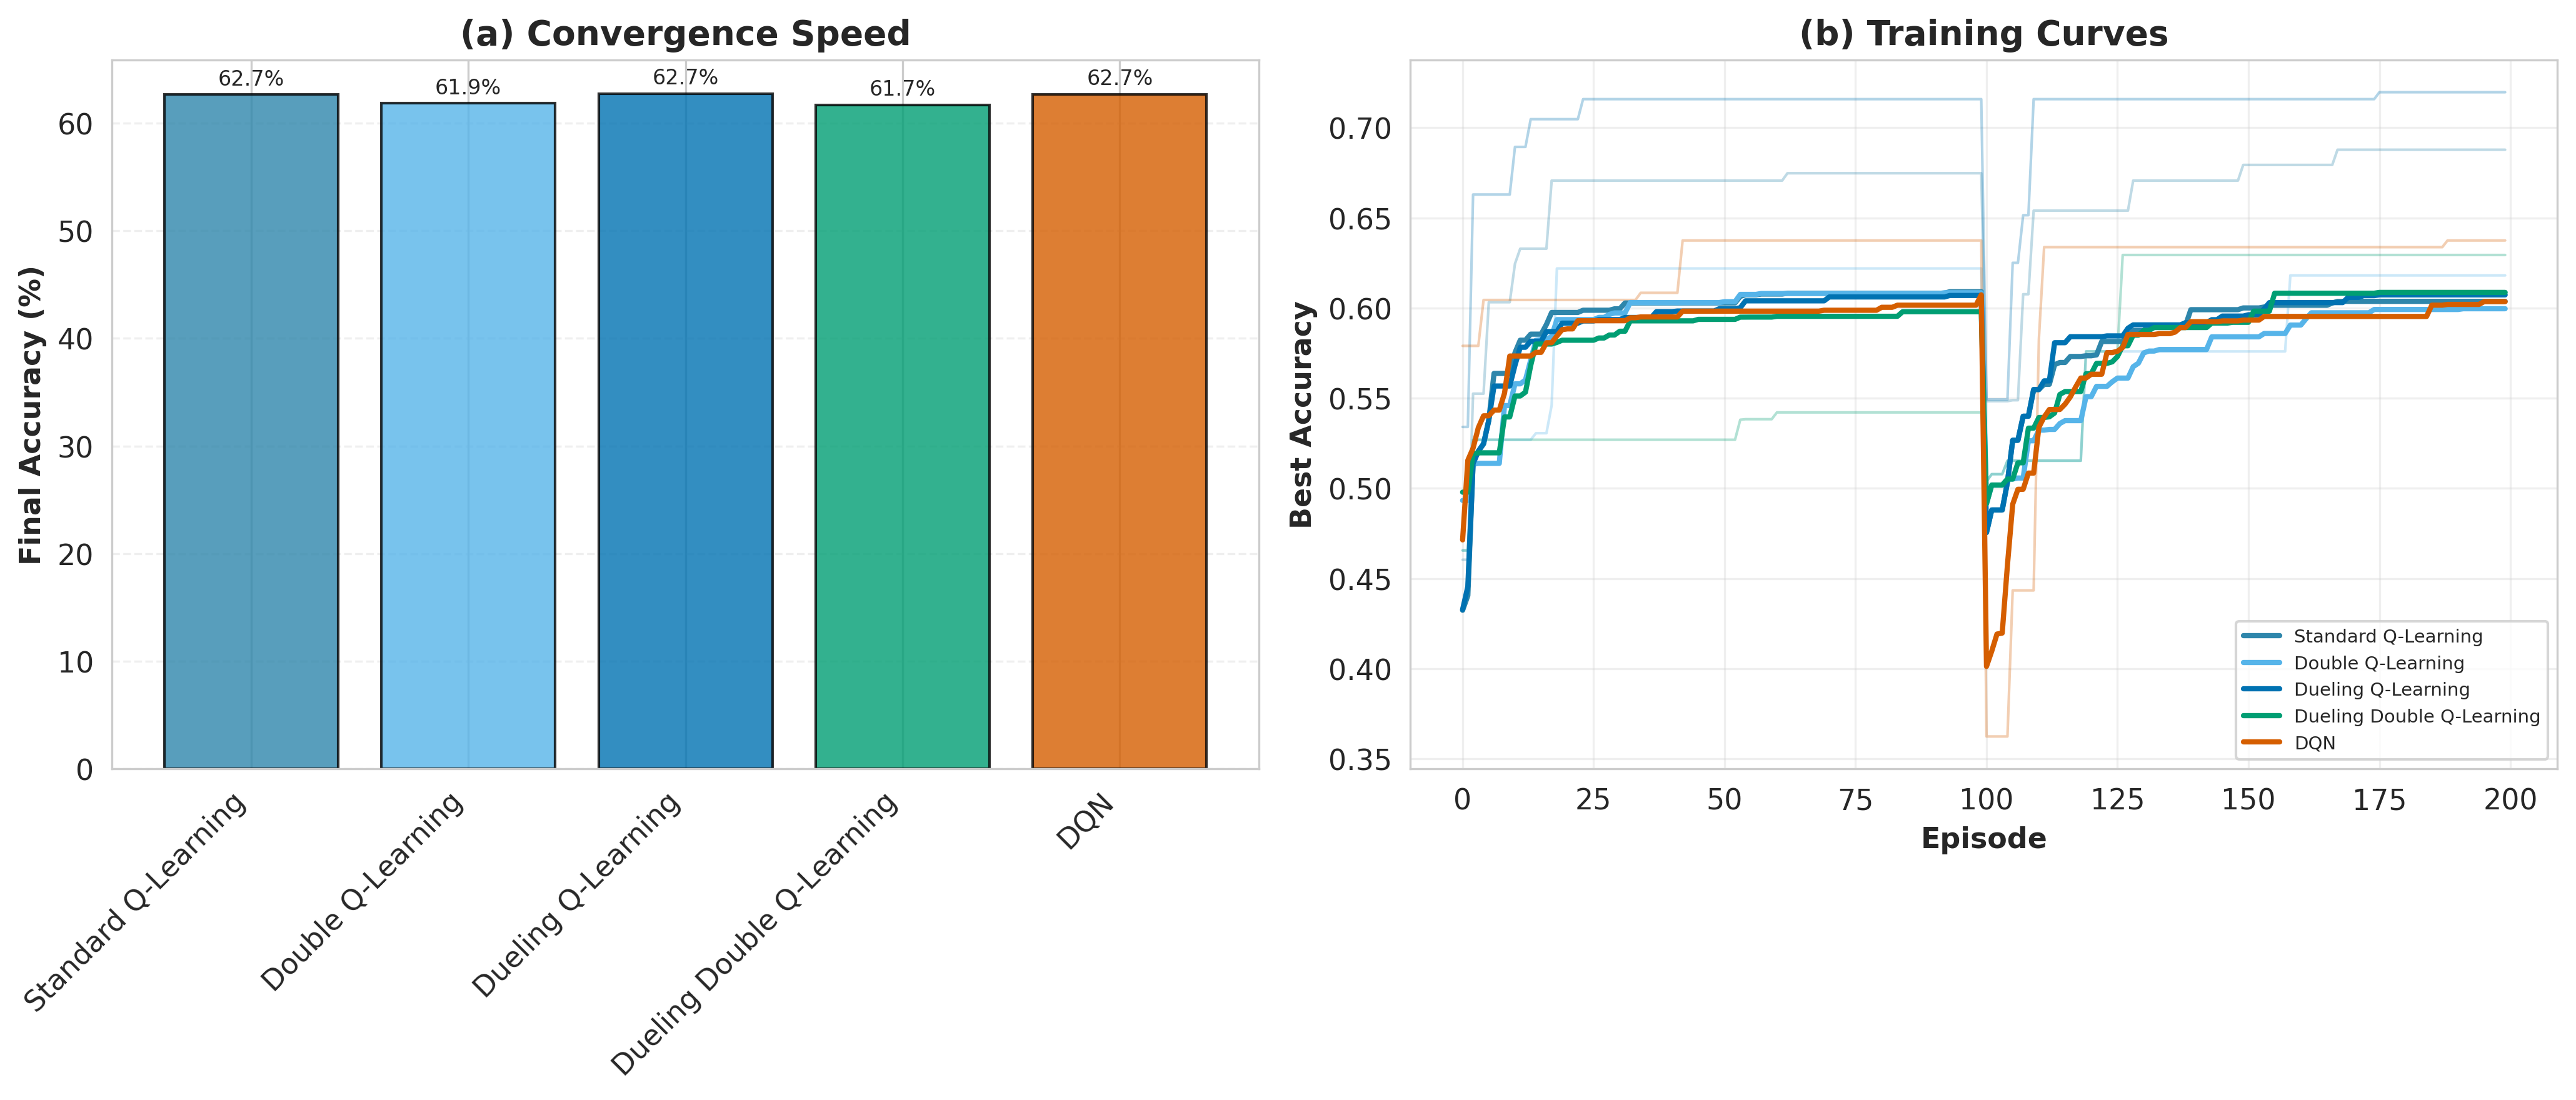
\includegraphics[width=0.85\textwidth]{figures/q_internal/03_training_performance.png}
    \end{center}
\end{frame}

\begin{frame}{训练收敛特性分析}
    \begin{exampleblock}{训练动态}
        \footnotesize
        \begin{itemize}
            \item \textbf{最终准确率}：Standard Q-Learning、Dueling Q-Learning 和 DQN 均达 62.7\%
            \item \textbf{收敛速度}：所有方法在 0--50 Episodes 快速收敛至 60\%
            \item \textbf{训练方差}：Double Q-Learning 方差大，Standard Q-Learning 和 DQN 更稳定
            \item \textbf{结论}：Standard Q-Learning 保持高性能同时，具有更优训练稳定性
        \end{itemize}
    \end{exampleblock}

    \vspace{0.2cm}
    \begin{alertblock}{结果分析}
        \footnotesize
        所有方法在初始阶段（0--50 Episodes）均表现出快速收敛特性，准确率迅速攀升至 60\% 左右。在 Episode 100 处观察到的性能波动后，各方法均能迅速恢复并趋于稳定。观察发现，Double Q-Learning 显示出较大的训练方差（细线离散度高），而 Standard Q-Learning 和 DQN 表现出更平滑、稳定的收敛过程。结果表明，Standard Q-Learning 在保持高性能的同时，具有更优的训练稳定性和收敛效率。
    \end{alertblock}
\end{frame}

\begin{frame}{Table Q-Learning vs DQN 详细对比}
    \begin{center}
    \footnotesize
    \renewcommand{\arraystretch}{1.1}
    \begin{tabular}{lcccc}
        \hline
        \textbf{Method} & \textbf{Accuracy (\%)} & \textbf{Kappa} & \textbf{F1} & \textbf{Std Dev (\%)} \\
        \hline
        Standard Q-Learning & \textbf{62.68 $\pm$ 8.20} & 0.502 & 0.620 & \textbf{8.20}  \\
        DQN & \textbf{62.70 $\pm$ 9.21} & 0.502 & 0.620 & 9.21  \\
        \textbf{$\Delta$ (Q - DQN)} & \textbf{-0.02} & -0.0003 & +0.0001 & \textbf{-1.01}  \\
        \hline
    \end{tabular}
    \end{center}
\end{frame}

\begin{frame}{Table Q-Learning vs DQN 结果分析}
    \begin{alertblock}{核心发现}
        \footnotesize
        \begin{itemize}
            \item \textbf{准确率差异}：仅 -0.02\%，统计上可忽略
            \item \textbf{稳定性}：Standard Q-Learning 标准差低 10.97\%
            \item \textbf{时间窗}：Standard Q-Learning 选择更短但信息密度更高的窗口
        \end{itemize}
    \end{alertblock}

    \vspace{0.2cm}
    \begin{exampleblock}{结果分析}
        \footnotesize
        \begin{enumerate}
            \item \textbf{准确率差异极小}：Standard Q-Learning 取得 62.68\% 的准确率，DQN 取得 62.70\% 的准确率，两者差异仅为 -0.02\%，在统计学上可忽略不计。
            \item \textbf{稳定性优势}：Standard Q-Learning 的标准差（8.20\%）低于 DQN（9.21\%），相对降低约 10.97\%。
            \item \textbf{时间窗选择差异}：Standard Q-Learning 选择的时间窗为 $[2.29\text{ s}, 3.17\text{ s}]$（窗口长度 0.88 s），DQN 选择的时间窗为 $[2.23\text{ s}, 3.28\text{ s}]$（窗口长度 1.05 s）。表格型方法倾向于选择更短但信息密度更高的时间窗。
        \end{enumerate}
    \end{exampleblock}
\end{frame}

\begin{frame}{被试级别性能对比}
    \begin{center}
    \footnotesize
    \renewcommand{\arraystretch}{1.1}
    \begin{tabular}{lcccccc}
        \hline
        \textbf{Subject} & \textbf{Table Q} & \textbf{DQN} & \textbf{$\Delta$} & \textbf{Table Q Kappa} & \textbf{DQN Kappa} & \textbf{$\Delta$} \\
        \hline
        S01 & 64.47 $\pm$ 2.35 & 65.71 $\pm$ 0.63 & -1.24 & 0.526 & 0.544 & -0.018 \\
        S02 & 58.37 $\pm$ 1.85 & 56.74 $\pm$ 2.58 & +1.63 & 0.478 & 0.423 & +0.055 \\
        S03 & 68.89 $\pm$ 3.70 & 71.70 $\pm$ 0.37 & -2.81 & 0.585 & 0.623 & -0.038 \\
        S04 & 51.91 $\pm$ 1.89 & 51.15 $\pm$ 1.52 & +0.76 & 0.359 & 0.347 & +0.012 \\
        S05 & 65.42 $\pm$ 0.63 & 65.27 $\pm$ 0.63 & +0.15 & 0.539 & 0.537 & +0.002 \\
        S06 & 47.03 $\pm$ 1.85 & 45.21 $\pm$ 1.83 & +1.82 & 0.295 & 0.263 & +0.033 \\
        S07 & 65.46 $\pm$ 0.19 & 65.61 $\pm$ 0.30 & -0.15 & 0.540 & 0.542 & -0.002 \\
        S08 & 73.56 $\pm$ 1.31 & 74.62 $\pm$ 0.00 & -1.06 & 0.647 & 0.661 & -0.014 \\
        S09 & 68.69 $\pm$ 1.06 & 68.27 $\pm$ 0.85 & +0.42 & 0.582 & 0.577 & +0.006 \\
        \hline
    \end{tabular}
    \end{center}
\end{frame}

\begin{frame}{被试级别性能分析}
    \begin{exampleblock}{被试分析}
        \footnotesize
        \begin{itemize}
            \item \textbf{优劣分布}：Table Q 在 5 名被试上优于或持平 DQN
            \item \textbf{低表现被试}：S06 上 Table Q 优于 DQN (+1.82\%)
            \item \textbf{高表现被试}：S03、S08 上 DQN 略优，差距 $< 3\%$
        \end{itemize}
    \end{exampleblock}

    \vspace{0.2cm}
    \begin{alertblock}{结果分析}
        \footnotesize
        \begin{enumerate}
            \item \textbf{性能优劣分布均衡}：在 9 名被试中，表格型 Q-Learning 在 5 名被试（S02、S04、S05、S06、S09）上优于或持平于 DQN，在 4 名被试（S01、S03、S07、S08）上略低于 DQN。
            \item \textbf{低表现被试上的优势}：在 S06 被试（低表现组）上，表格型 Q-Learning 取得 47.03\% 的准确率，优于 DQN 的 45.21\%（$\Delta = +1.82\%$）。
            \item \textbf{高表现被试上的差距}：在 S03 和 S08 被试（高表现组）上，DQN 略优于表格型方法，但差距在可接受范围内（$< 3\%$）。
        \end{enumerate}
    \end{alertblock}
\end{frame}

\begin{frame}{统计显著性检验}
    \begin{alertblock}{配对样本$t$检验结果}
        \footnotesize
        \begin{itemize}
            \item \textbf{假设}：$H_0: \mu_d = 0$ (无显著差异) vs $H_1: \mu_d \neq 0$
            \item \textbf{$t$统计量}：$t(8) = -0.024$
            \item \textbf{$p$值}：$p = 0.981 > 0.05$
            \item \textbf{95\% CI}：$[-2.01\%, 1.97\%]$
            \item \textbf{效应量}：Cohen's $d = -0.003$
        \end{itemize}
    \end{alertblock}

    \vspace{0.2cm}
    \begin{exampleblock}{结果解读}
        \footnotesize
        \begin{itemize}
            \item $p = 0.981 > 0.05$，不能拒绝零假设
            \item 效应量$d = -0.003$远小于 0.2 阈值
            \item \textbf{核心主张验证}：表格型 Q-Learning 可在不显著牺牲性能前提下替代 DQN
        \end{itemize}
    \end{exampleblock}
\end{frame}

% ============================================================================
% Q-Learning 变体消融实验
% ============================================================================
\subsection{消融实验}

\begin{frame}{Q-Learning 改进策略消融实验}
    \begin{center}
    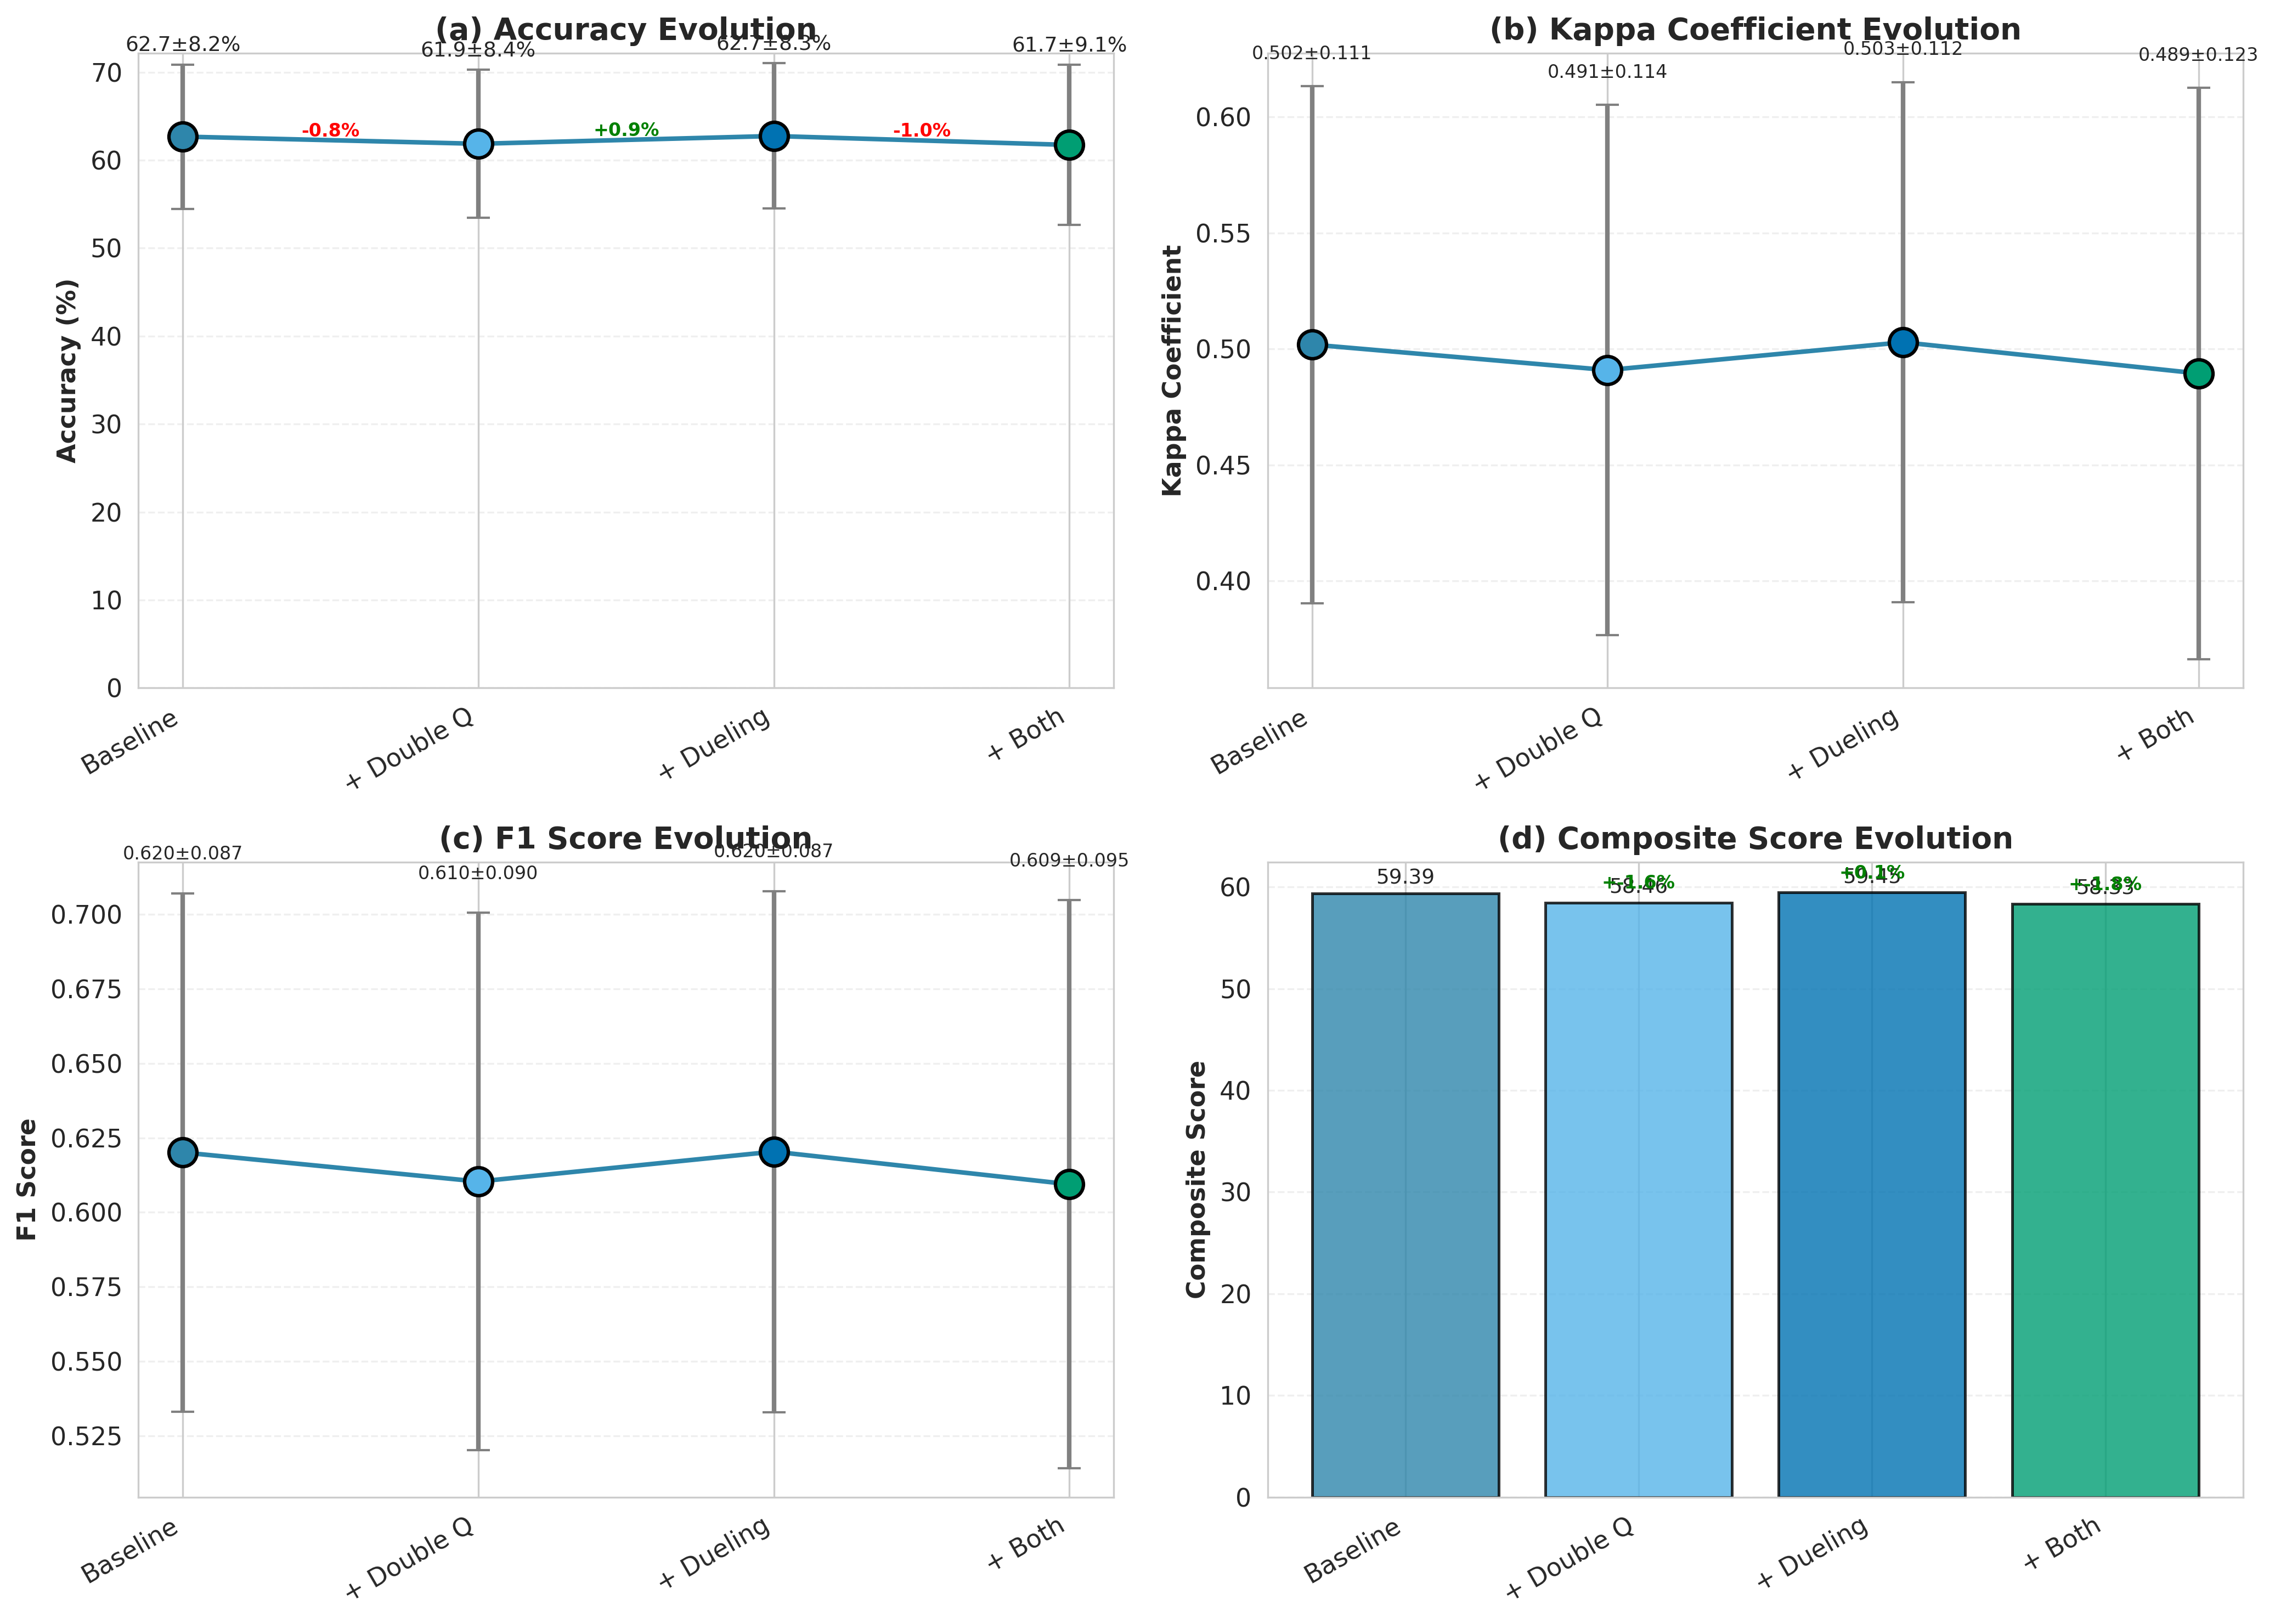
\includegraphics[width=0.85\textwidth]{figures/ablation/04_performance_evolution.png}
    \end{center}
\end{frame}

\begin{frame}{Q-Learning 改进策略消融实验分析}
    \begin{alertblock}{性能演变}
        \footnotesize
        \begin{itemize}
            \item \textbf{Baseline}：62.7\% 准确率
            \item \textbf{+ Double Q}：下降至 61.9\% (-0.8\%)
            \item \textbf{+ Dueling}：恢复至 62.7\% (+0.9\%)
            \item \textbf{+ Both}：略降至 61.7\% (-1.0\%)
            \item \textbf{结论}：Dueling 架构维持性能，Double Q 未带来预期收益
        \end{itemize}
    \end{alertblock}

    \vspace{0.2cm}
    \begin{exampleblock}{结果分析}
        \footnotesize
        Baseline 准确率为 62.7\%，引入 Double Q 后略微下降至 61.9\% (-0.8\%)，引入 Dueling 架构后恢复至 62.7\% (+0.9\%)，而两者结合（Dueling Double Q-Learning）略降至 61.7\% (-1.0\%)。Kappa 系数和 F1 分数趋势与准确率一致，Baseline (0.502) 与 + Dueling (0.503) 表现最佳，涉及 Double Q 的变体略低（0.491 和 0.489）。结果表明，在本任务中，\textbf{Dueling 架构能维持基线性能，但 Double Q 机制并未带来预期收益}，Standard Q-Learning 已是最优选择。
    \end{exampleblock}
\end{frame}

\begin{frame}{时间窗口选择演变分析}
    \begin{center}
    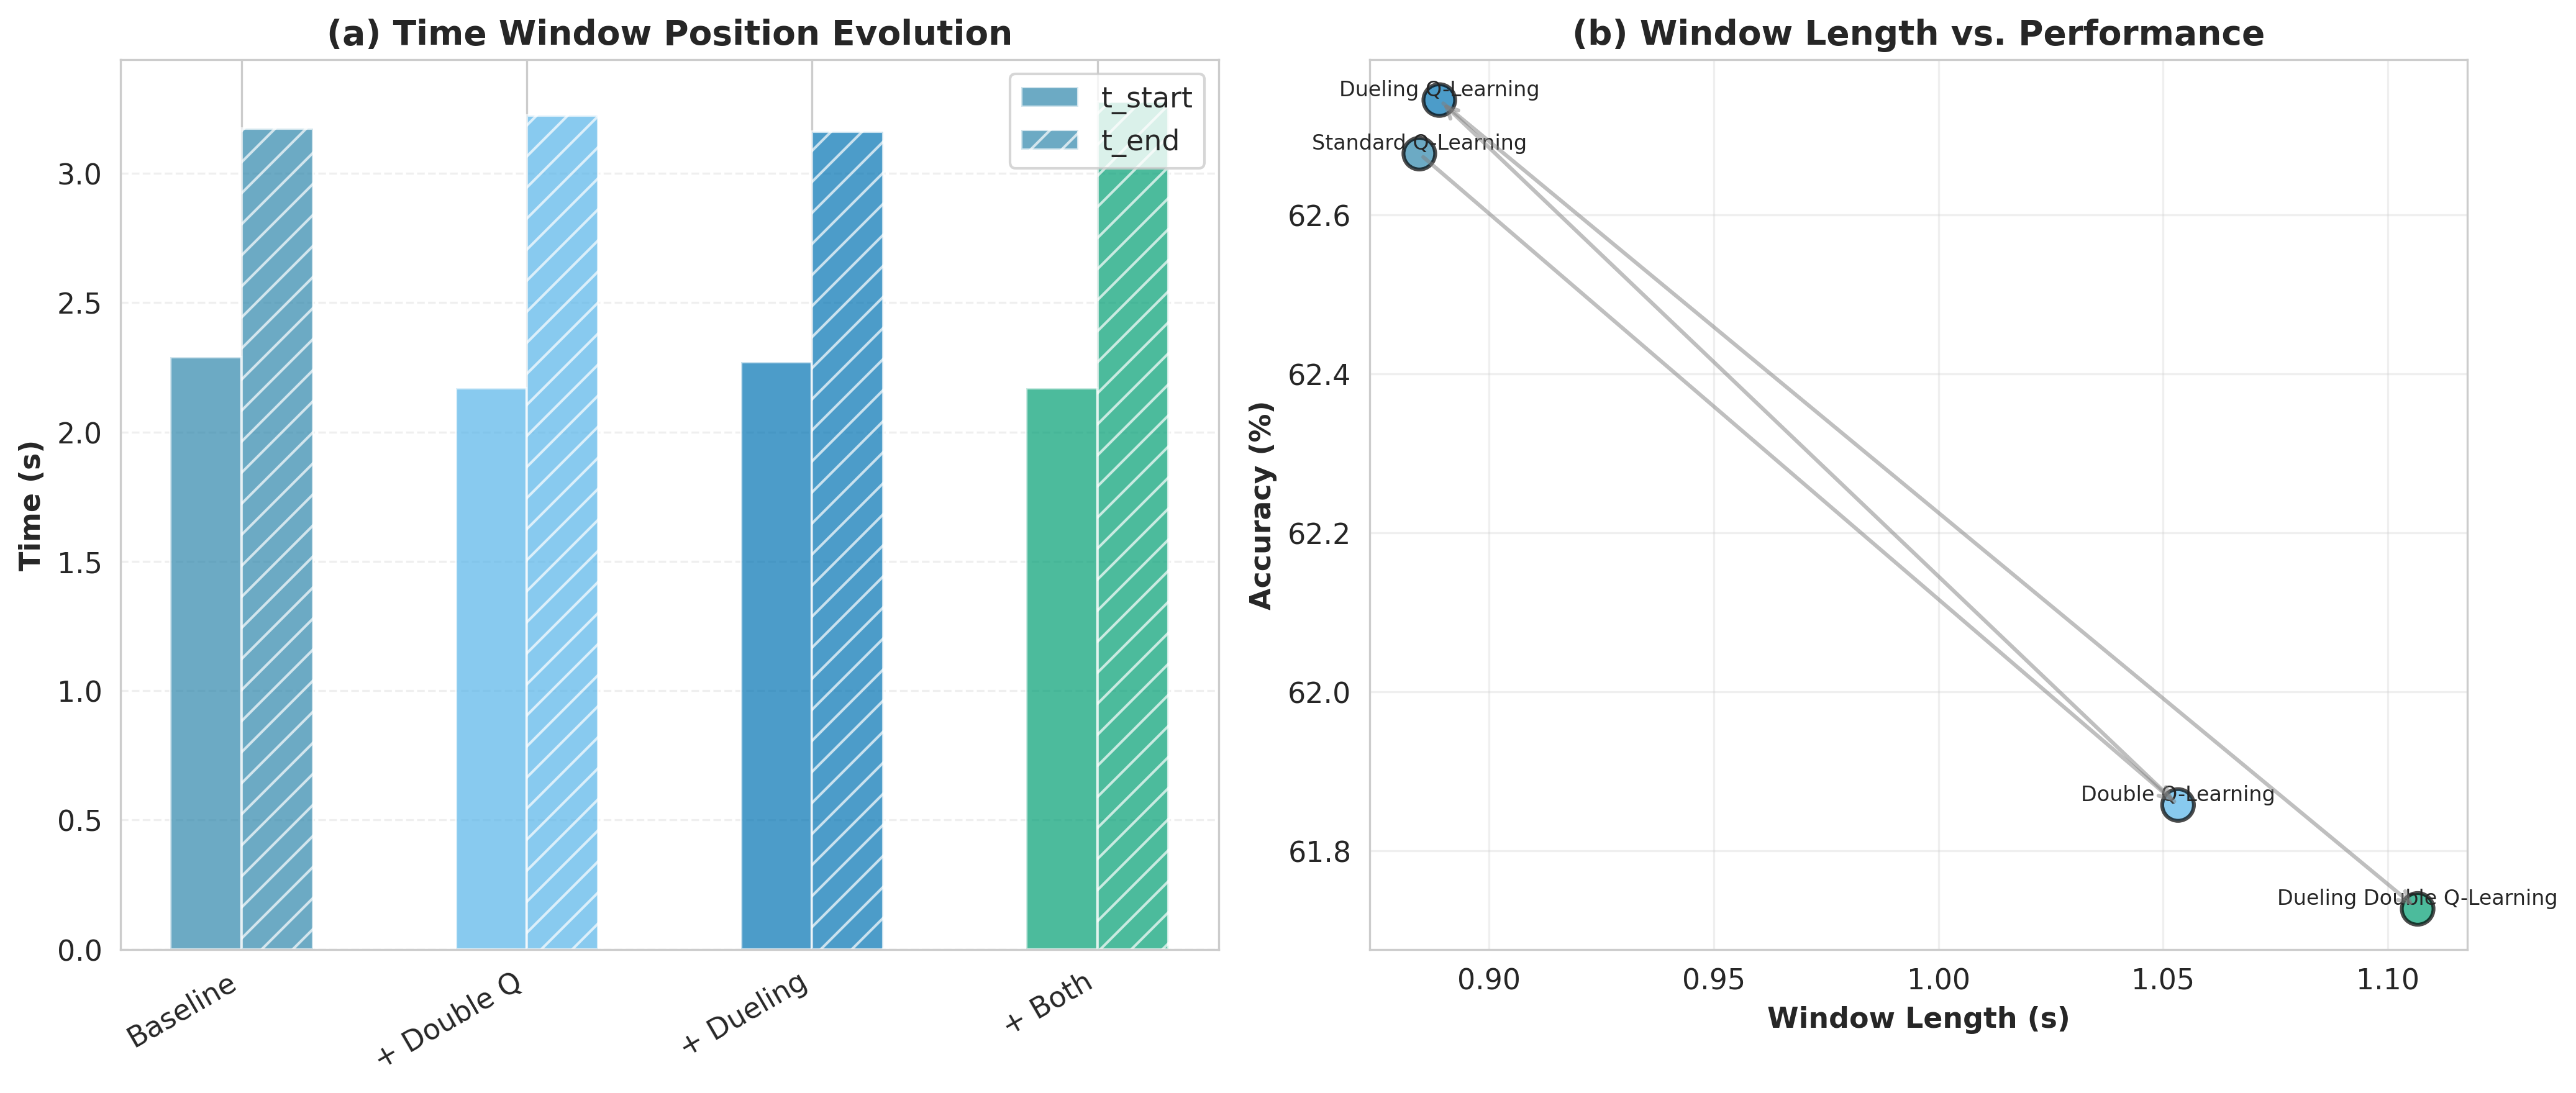
\includegraphics[width=0.85\textwidth]{figures/ablation/04_window_evolution.png}
    \end{center}
\end{frame}

\begin{frame}{时间窗口选择演变分析}
    \begin{exampleblock}{窗口模式}
        \footnotesize
        \begin{itemize}
            \item \textbf{位置}：所有方法一致选择后期片段 (起始约 2.2s，结束约 3.3s)
            \item \textbf{窗口长度与性能}：显著负相关
            \item \textbf{Standard/Dueling Q}：短窗口 (0.9s)，高准确率 (62.7\%)
            \item \textbf{Double Q 变体}：长窗口 (1.05s--1.1s)，略低准确率 (61.7\%--61.9\%)
            \item \textbf{结论}：精简窗口 (0.9s) 更利于捕捉判别性特征
        \end{itemize}
    \end{exampleblock}

    \vspace{0.2cm}
    \begin{alertblock}{结果分析}
        \footnotesize
        所有方法均一致地选择试验后期的时间片段（起始约 2.2s，结束约 3.2s--3.3s），验证了运动想象关键特征分布的时间稳定性。窗口长度与分类准确率的关系散点图显示显著的负相关趋势：Standard Q-Learning 和 Dueling Q-Learning 选择了较短的窗口（约 0.9s），取得了更高的准确率（62.7\%）；而引入 Double Q 机制的变体倾向于选择较长的窗口（1.05s--1.1s），准确率略低（61.7\%--61.9\%）。这表明\textbf{精简的时间窗口（约 0.9s）更有利于捕捉判别性特征并抑制噪声干扰}。
    \end{alertblock}
\end{frame}

\begin{frame}{改进策略详细分析}
    \begin{center}
    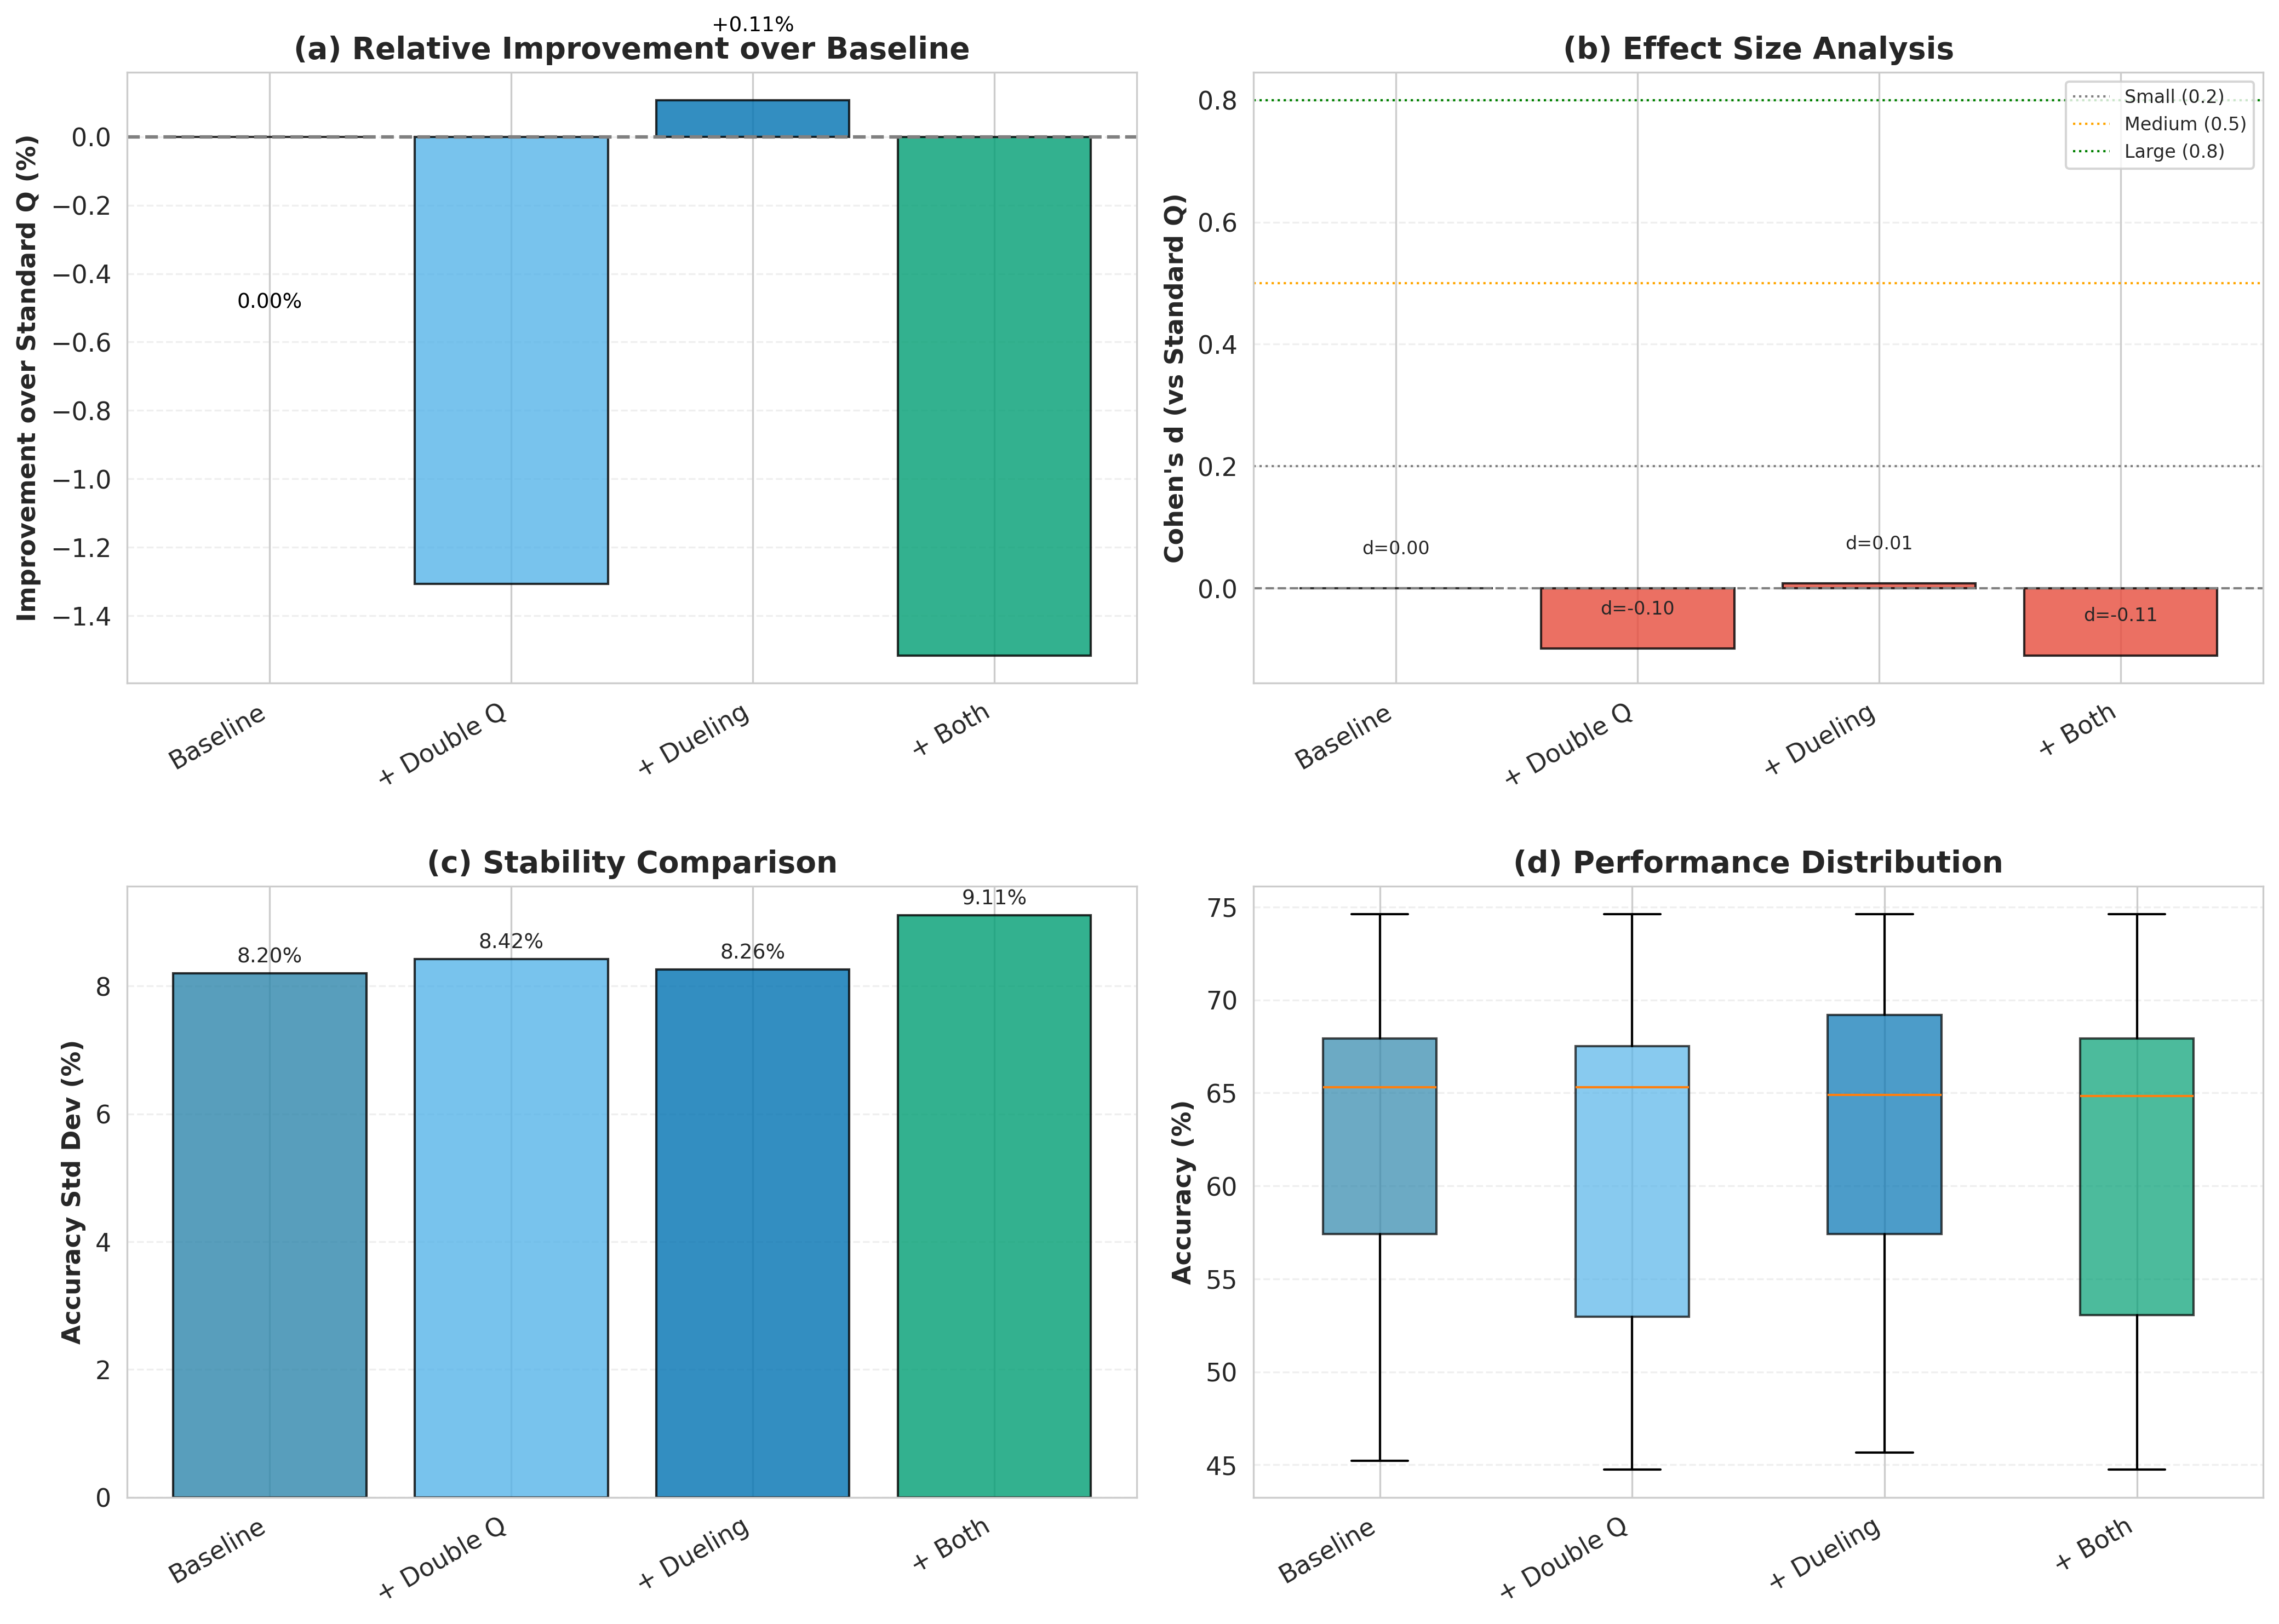
\includegraphics[width=0.85\textwidth]{figures/ablation/04_improvement_analysis.png}
    \end{center}
\end{frame}

\begin{frame}{改进策略详细分析}
    \begin{alertblock}{综合分析}
        \footnotesize
        \begin{itemize}
            \item \textbf{相对提升}：Dueling (+0.11\%)，Double Q (-1.3\%)，Both (-1.5\%)
            \item \textbf{效应量}：所有$|d| < 0.2$，Double Q 和 Both 显示微小负效应
            \item \textbf{稳定性}：Baseline 最优 (8.20\%)，Both 波动最大 (9.11\%)
            \item \textbf{结论}：Standard Q-Learning 已是最优选择，复杂机制增加开销
        \end{itemize}
    \end{alertblock}

    \vspace{0.2cm}
    \begin{exampleblock}{结果分析}
        \footnotesize
        Dueling 架构带来了微小的正向提升（+0.11\%），而引入 Double Q 机制（-1.3\%）及两者结合（Both, -1.5\%）均导致性能下降。所有变体与基线的效应量均远小于小效应阈值（$|d| < 0.2$）。Baseline 表现出最佳的稳定性（Std Dev = 8.20\%），而 + Both 的波动性最大（9.11\%）。综合分析表明，\textbf{Standard Q-Learning 已足以有效解决本任务的时间窗口选择问题}，引入 Double Q 或 Dueling 等复杂机制不仅未能提升性能，反而可能增加计算复杂度并略微降低稳定性。
    \end{exampleblock}
\end{frame}

\begin{frame}{消融实验详细对比}
    \begin{center}
    \footnotesize
    \renewcommand{\arraystretch}{1.3}
    \begin{tabular}{lcccc}
        \hline
        \textbf{Method} & \textbf{Accuracy (\%)} & \textbf{Kappa} & \textbf{F1} & \textbf{Std Dev (\%)} \\
        \hline
        Baseline (Standard Q) & \textbf{62.68 $\pm$ 8.20} & 0.502 & 0.620 & \textbf{8.20} \\
        + Double Q & 61.86 $\pm$ 8.42 & 0.491 & 0.610 & 8.42 \\
        + Dueling & 62.74 $\pm$ 8.26 & 0.503 & 0.620 & 8.26 \\
        + Both & 61.73 $\pm$ 9.11 & 0.489 & 0.609 & 9.11 \\
        \hline
    \end{tabular}
    \end{center}
\end{frame}

\begin{frame}{消融实验结论}
    \begin{exampleblock}{消融结论}
        \footnotesize
        \begin{itemize}
            \item Standard Q-Learning 在准确率和稳定性上均表现最优
            \item Double Q 机制导致性能下降 (-0.82\%) 和稳定性降低
            \item Dueling 架构维持基线性能，但无显著提升
            \item \textbf{最终选择}：Standard Q-Learning 为本任务最优方案
        \end{itemize}
    \end{exampleblock}
\end{frame}

% ============================================================================
% 本章小结
% ============================================================================
\subsection{本章小结}

\begin{frame}{本章小结}
    \begin{alertblock}{实验结论}
        \footnotesize
        \begin{itemize}
            \item \textbf{基线对比}：搜索优化方法 (63.3\%) 显著优于固定窗口 (45\%)
            \item \textbf{Q-Learning vs 基线}：性能相当 (62.7\% vs 63.3\%)，差异不显著
            \item \textbf{Table Q-Learning vs DQN}：准确率差异仅 -0.02\% ($p=0.981$)
            \item \textbf{消融实验}：Standard Q-Learning 为最优选择
        \end{itemize}
    \end{alertblock}

    \vspace{0.2cm}
    \begin{exampleblock}{核心验证}
        \footnotesize
        \begin{itemize}
            \item 表格型 Q-Learning 可在不显著牺牲性能前提下替代 DQN
            \item 稳定性优于 DQN (标准差降低 10.97\%)
            \item 推理效率$O(1)$查表，满足实时 BCI 要求
        \end{itemize}
    \end{exampleblock}
\end{frame}

} % end of \small
